\chapter{Results}
\label{cha:results}

This chapter reports the results of several real world instances of Makahiki implemented in different organizations, as well as the the application of SGSEAM to the Makahiki framework.

\section{Real-World Case Studies}
\label{sec:realworld-result}

We used Makahiki to create a total of seven Kukui Cup Energy Challenges in four different organizations. The following sections describe the Makahiki instances for the four organizations and the different configurations for these instances.

\subsection{Makahiki instances}

\subsubsection{University of Hawaii at Manoa}

There were three instances of Kukui Cup (KC) Challenges implemented by using the Makahiki framework at the University of Hawaii at Manoa (UHM). They were held in 2011, 2012, and 2014 respectively for over 1000 first year students per year living in the residence halls on campus. The three instances had competition durations of 3 weeks, 9 months and 2 weeks respectively. The residence halls where the students were living had energy smart meters installed for collecting the energy data consumed by the students. 

\begin{figure}[ht!]
   \centering
   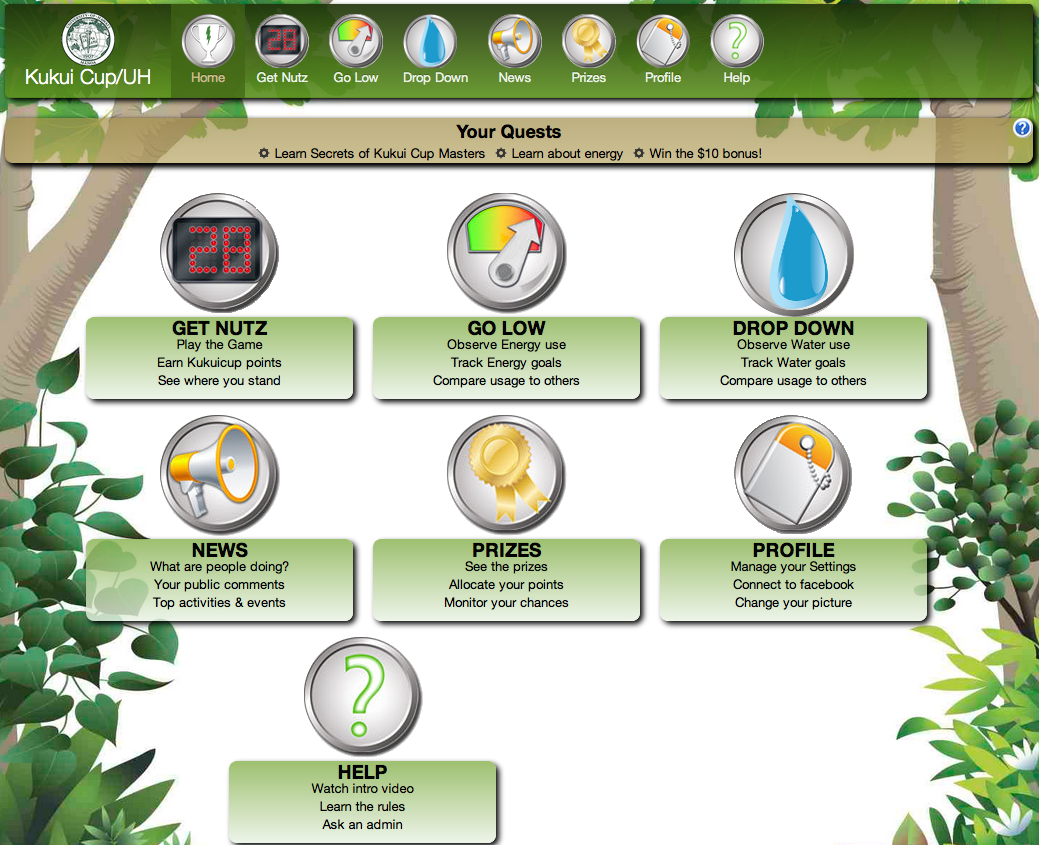
\includegraphics[width=20em]{uhm-homepage}
   \caption{UHM Kukui Cup Challenge Home Page}
   \label{fig:uhm-homepage}
\end{figure}

\subsubsection{Hawaii Pacific University}

There were two instances of Kukui Cup Challenges implemented using the Makahiki framework at Hawaii Pacific University (HPU). They were held in 2012 and 2013 respectively for about 200 students per year living in 6 residence halls at the Hawaii Loa Campus. Energy smart meters were installed in the residence halls.

\begin{figure}[ht!]
   \centering
   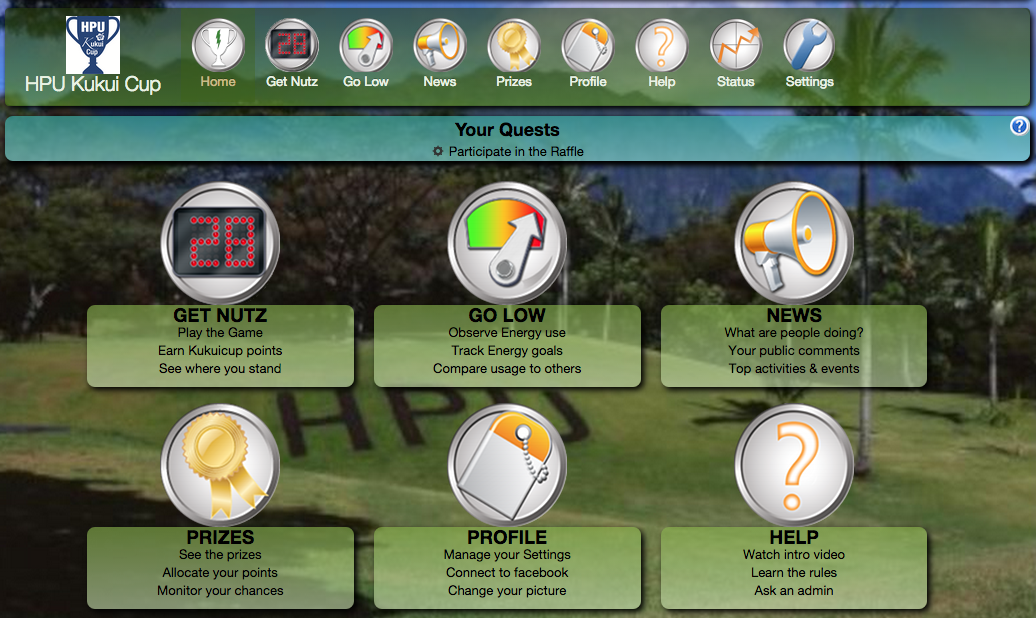
\includegraphics[width=20em]{hpu-homepage}
   \caption{HPU Kukui Cup Challenge Home Page}
   \label{fig:hpu-homepage}
\end{figure}

\subsubsection{East-West Center}

The EWC Kukui Cup Energy and Water challenge was implemented by an international organization called the East-West Center (EWC) using the Makahiki framework. It was held in 2012 for approximately 600 international students living in two residence halls in Hawaii. The challenge lasted for 2 weeks and includes energy and water saving competition between two residence halls. The residence halls did not have internet-enabled smart meters, so energy data was collected by program organizers by reading the meters each day at the same time and entering the readings into the system manually.

\begin{figure}[ht!]
   \centering
   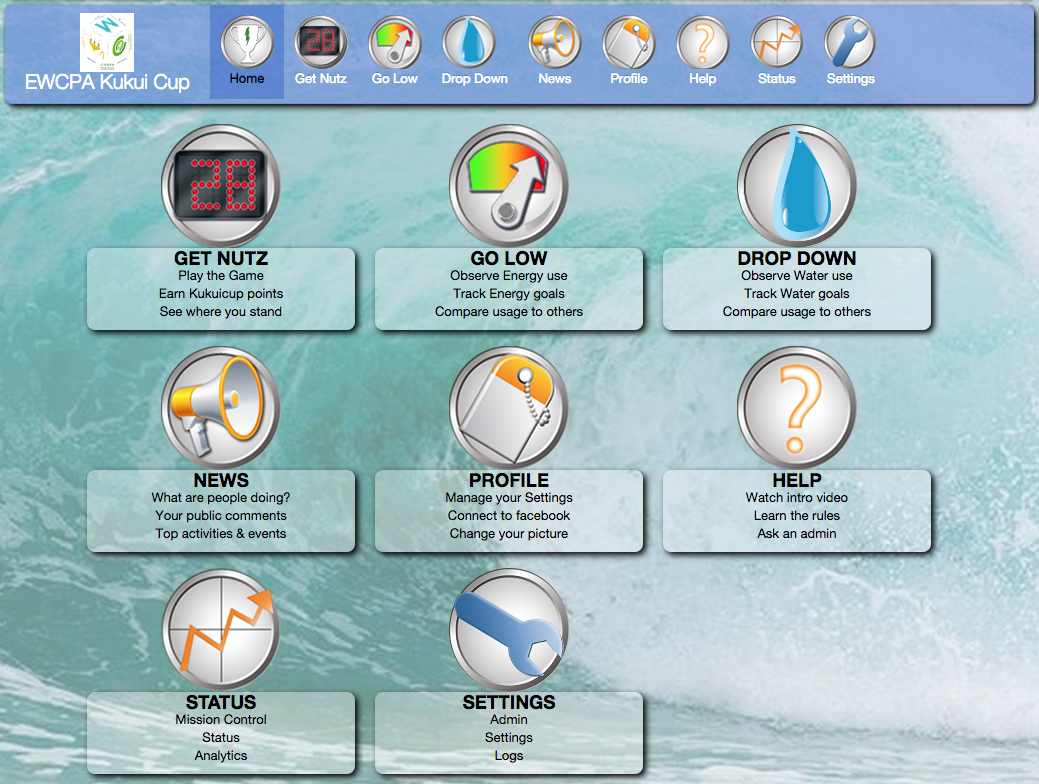
\includegraphics[width=20em]{ewc-homepage}
   \caption{EWC Kukui Cup Challenge Home Page}
   \label{fig:ewc-homepage}
\end{figure}

\subsubsection{Holy Nativity School}

A pilot instance of Kukui Cup challenge implemented by using the Makahiki framework was held at the Holy Nativity School (HNS), a private elementary school in Hawaii, in 2013. The pilot instance was organized by the school with the partnership with Project Learning Tree (PLT) GreenSchool! program\cite{plt-greenschools}. This nationwide environmental service-learning program helps improve student academic performance in STEM subjects by addressing environmental issues at their school. This challenge was designed so that it did not require any energy or water data. It was used to supplement STEM education with a sustainability focus. The challenge was initially scheduled for one month. It was later extended to 7 months.

\begin{figure}[ht!]
   \centering
   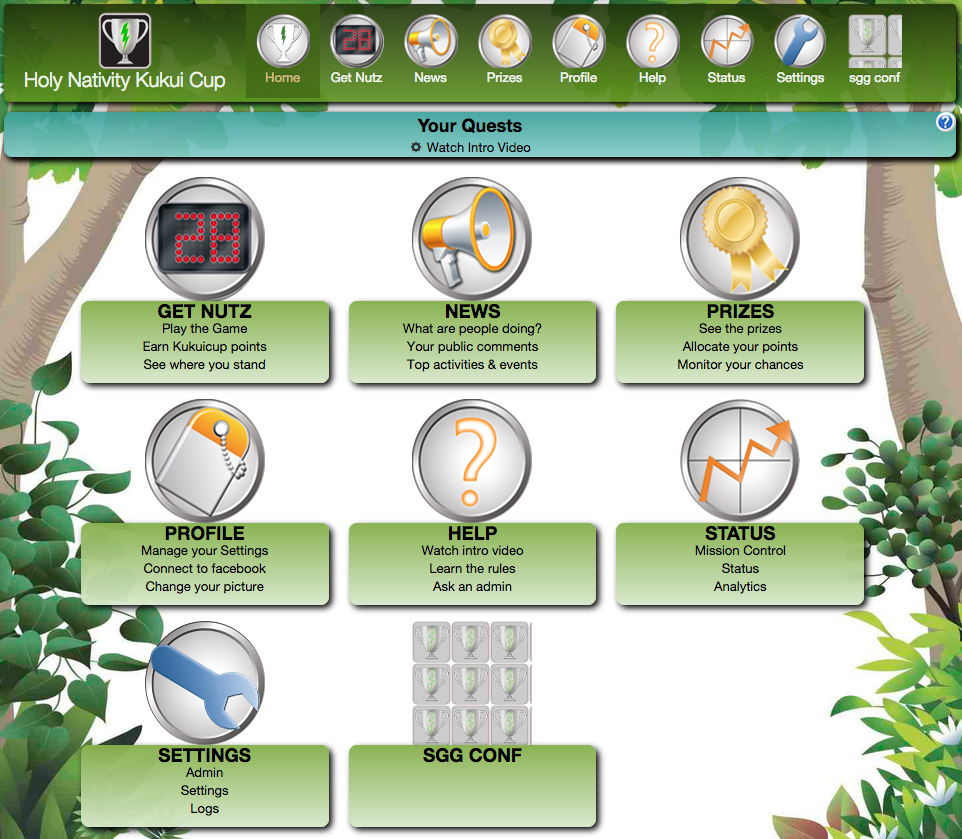
\includegraphics[width=20em]{hns-homepage}
   \caption{HNS Kukui Cup Challenge Home Page}
   \label{fig:hns-homepage}
\end{figure}

\subsection{Customization of the Makahiki Instances}

The following sections describe the different customizations that were done to the above Makahiki instances to address each  organization's needs.

\subsubsection{Challenge Customization}
Challenge customization includes the duration of the challenge, the participant accounts, resource customization such as energy and water settings, learning action configuration, prize and other game mechanics settings. 

\autoref{table:challenge-configurations} lists the different configurations between the seven real world instances of Makahiki.

\begin{table}[ht!]
  \centering
  \begin{tabular} {|c|c|c|c|c|c|c|c|c|}
    \hline
    \tabhead{Instances} &
    \tabhead{Participants} &
    \tabhead{Teams} &
    \tabhead{Duration} &
    \tabhead{Rounds} &
    \multicolumn{4}{c|}{\tabhead{Game Element}} \\
    \cline{6-9}
    & & & & &     
    \tabhead{Energy} &
    \tabhead{Water} &
    \tabhead{Prize} &
    \tabhead{Quest} \\
    \hline
    UHM2011 & 1070 & 20 & 3 weeks & 3 & \checkmark &  & \checkmark & \checkmark\\
    \hline
    UHM2012 & 1086 & 20 & 9 months & 4 & \checkmark &  & \checkmark & \checkmark\\
    \hline
    UHM2014 & 1093 & 20 & 2 weeks & 2 & \checkmark &  & \checkmark & \checkmark\\
    \hline
    HPU2012 & 189 & 6 & 3 weeks & 3 & \checkmark &  & \checkmark & \checkmark\\
    \hline
    HPU2013 & 197 & 6 & 3 weeks & 3 & \checkmark &  & \checkmark & \checkmark\\
    \hline
    EWC2012 & 130 & 2 & 2 weeks & 1 & \checkmark  & \checkmark &  & \\
    \hline
    HNS2013 & 10 & 2 & 7 months & 1 &  &  & \checkmark & \checkmark \\
    \hline
  \end{tabular}
  \caption{Challenge Configuration Differences}
  \label{table:challenge-configurations}
\end{table}

As we can see from the \autoref{table:challenge-configurations}, the Makahiki framework can be customized to support different numbers of participants, different team sizes, different durations, different numbers of rounds, and different types of game elements.  For example, while the UHM and HPU
challenges involved only energy consumption data, the EWC challenge involved both energy
and water consumption data. 

\subsubsection{Content Customization}
Because different organizations have different sustainability education needs, they used the Makahiki framework to customize the content, which is shown to players via the SmartGrid Game. They can re-use or modify the existing contents included with the Makahiki framework or create new content to be included in the system. \autoref{table:sgg-configurations} shows the differences in  type and layout of educational contents. UHM had the most number of learning actions while HNS has the least. 

\begin{table}[ht!]
  \centering
  \begin{tabular} {|c|c|c|c|c|c|c|}
    \hline
    \tabhead{Instances} &
    \tabhead{Levels} &
    \tabhead{Activities} &
    \tabhead{Commitments} &
    \tabhead{Events} & 
    \tabhead{Total Actions}\\
    \hline
    UHM2011 & 1 & 51 & 21 & 21  & 93 \\
    \hline
    UHM2012 & 7 & 68 & 23 & 35  & 126 \\
    \hline
    UHM2014 & 4 & 60 & 21 & 20  & 101\\
    \hline
    HPU2012 & 3 & 24 & 11 & 4  & 39 \\
    \hline
    HPU2013 & 3 & 29 & 11 & 4  & 44 \\
    \hline
    EWC2012 & 4 & 21 & 1 & 19  & 41 \\
    \hline
    HNS2013 & 2 & 22 & 6 & 4  & 32 \\
    \hline
  \end{tabular}
  \caption{Content Differences}
  \label{table:sgg-configurations}
\end{table}

The layout of the educational content represented in the SmartGrid game is also highly customizable to include different levels, rows and columns. The figures  \autoref{fig:UHM-SGG}, \autoref{fig:HPU-SGG}, \autoref{fig:EWC-SGG}, \autoref{fig:GS-SGG} illustrate the content and layout of the educational SmartGrid game in the different Makahiki instances. 

\begin{figure}[http]
	\centering
		\subfigure[UHM 2011 Kukui Cup SmartGrid Game]{\label{fig:uh-2011}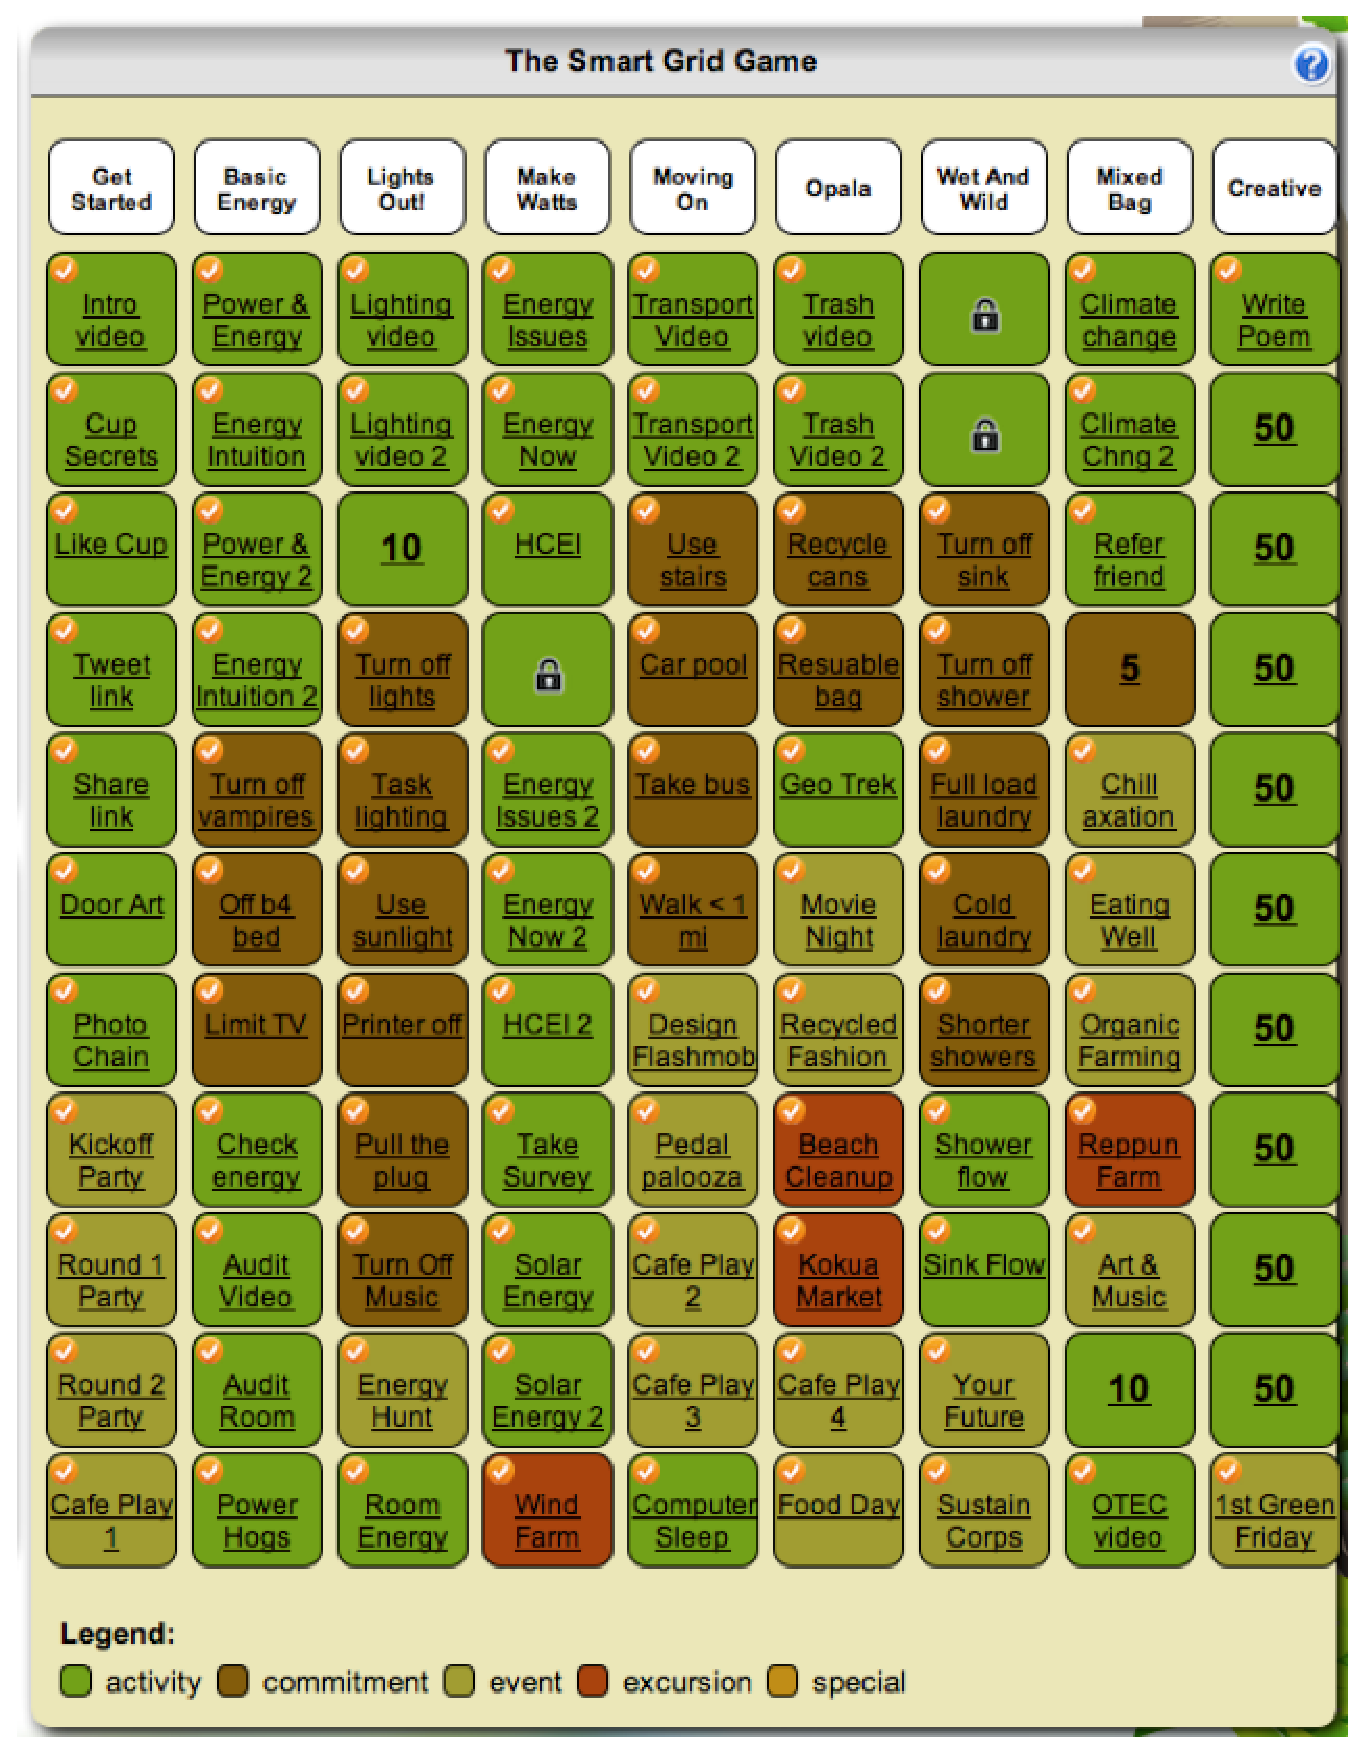
\includegraphics[height=3.6in,width=3.5in]{UH-SGG-2011.eps}}
		\subfigure[UHM 2012 Kukui Cup SmartGrid Game]{\label{fig:uh-2012}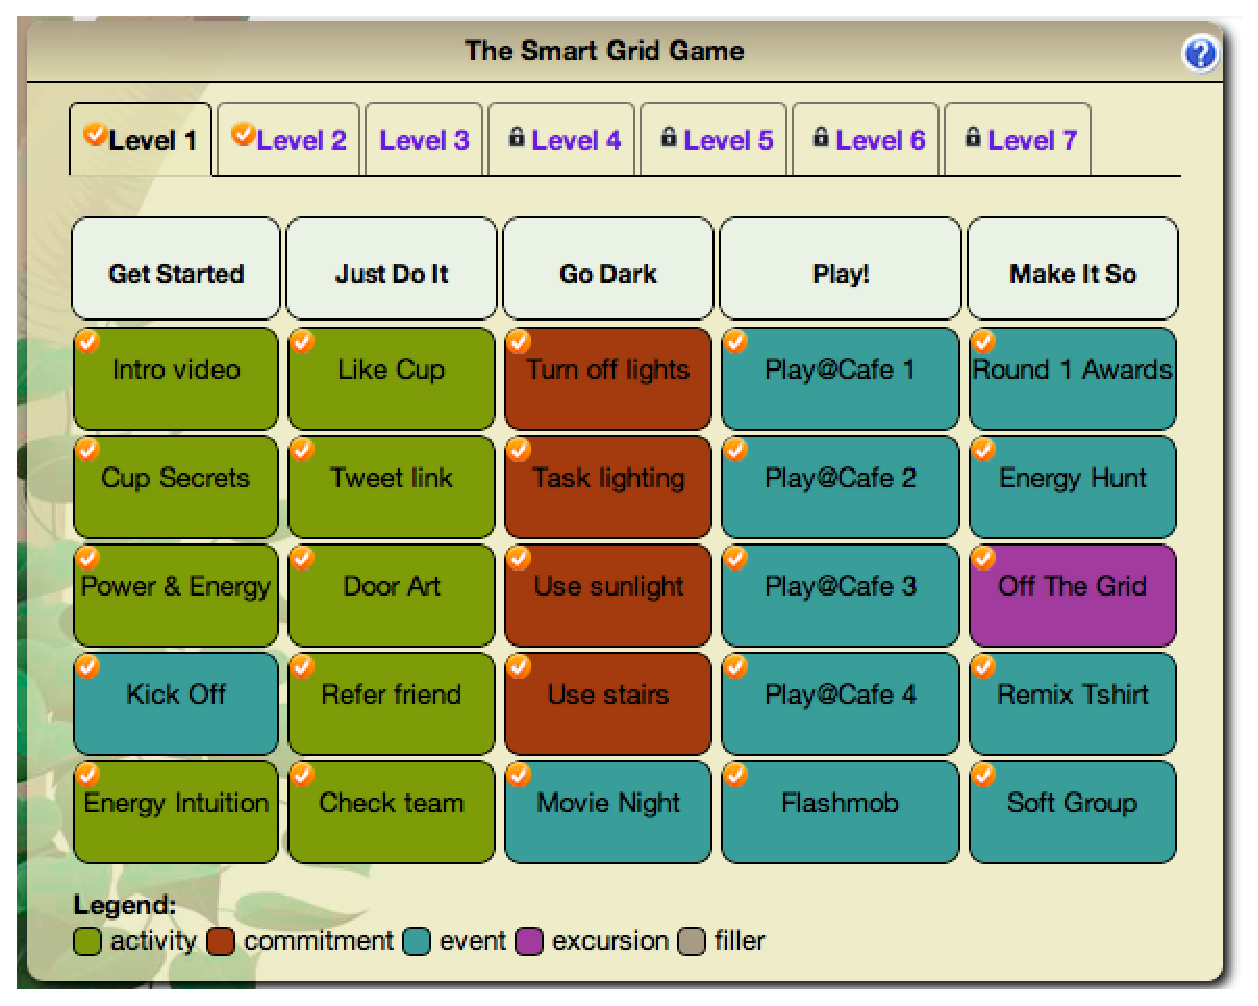
\includegraphics[height=1.8in,width=3.5in]{UH-SGG-2012.eps}}
		\subfigure[UHM 2014 Kukui Cup SmartGrid Game]{\label{fig:uh-2014}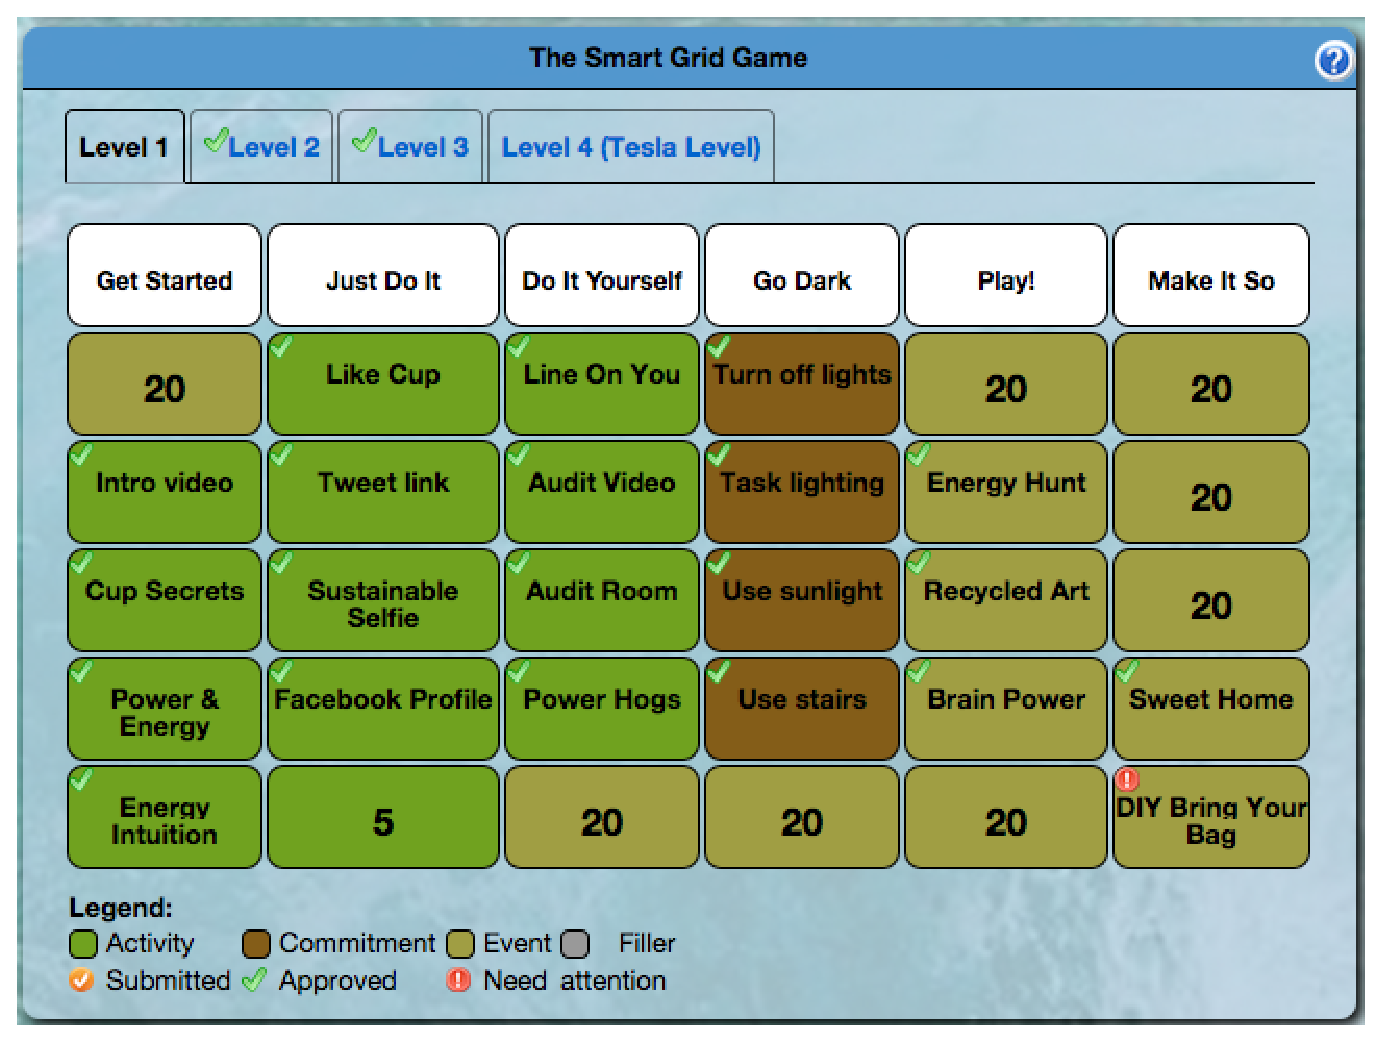
\includegraphics[height=1.8in,width=3.5in]{UH-SGG-2014.eps}}
		\caption{UHM SmartGrid Game Layouts}
		\label{fig:UHM-SGG}
\end{figure}

\begin{figure}[htbp]
	\centering
		\subfigure[HPU SmartGrid Game Level1]{\label{fig:hpu-level1}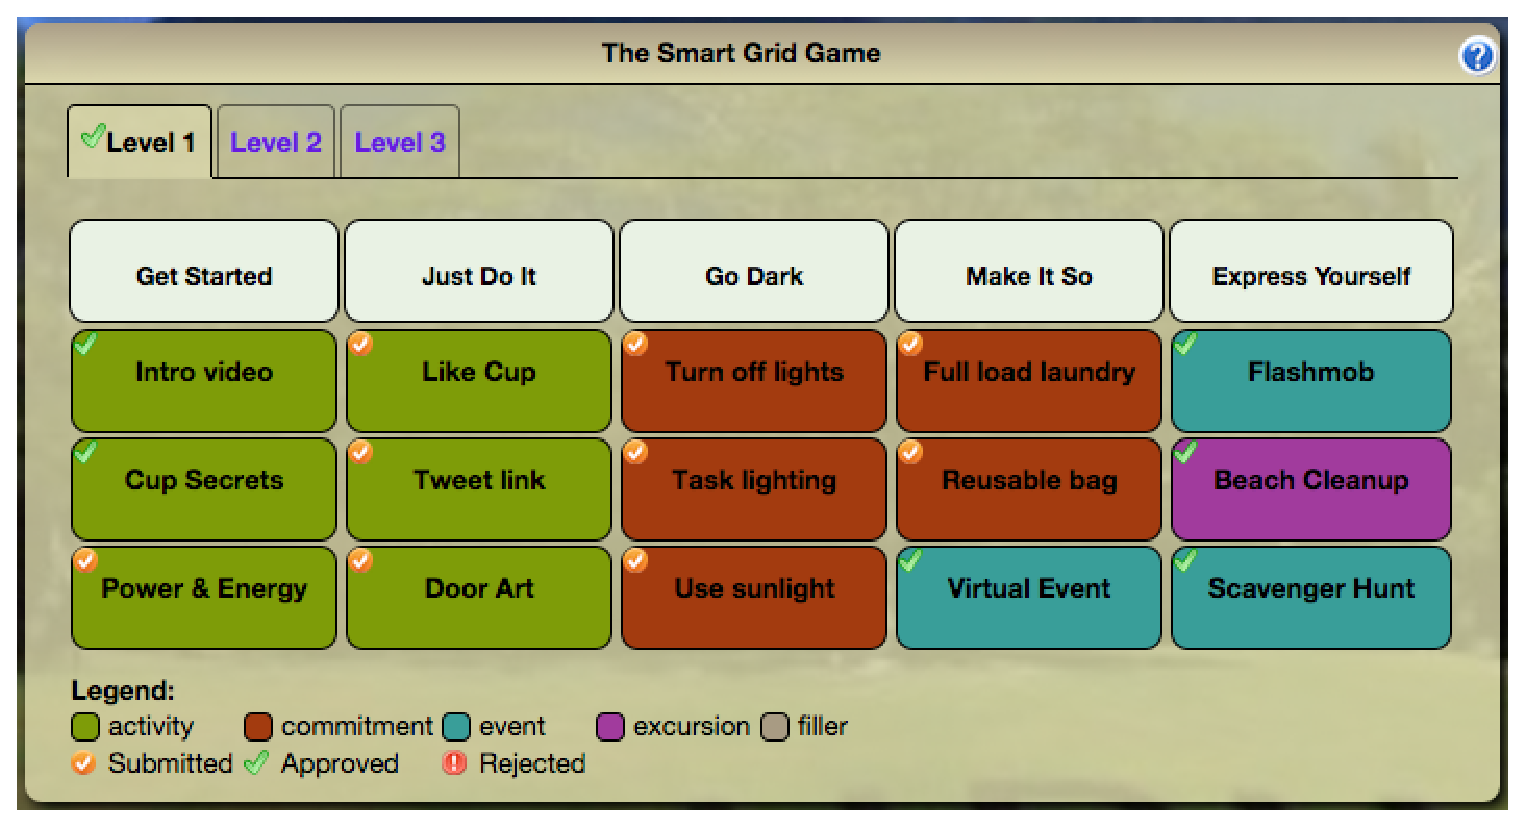
\includegraphics[height=2in,width=3.5in]{HPU-SGG-level1.eps}}
		\subfigure[HPU SmartGrid Game Level2]{\label{fig:hpu-level2}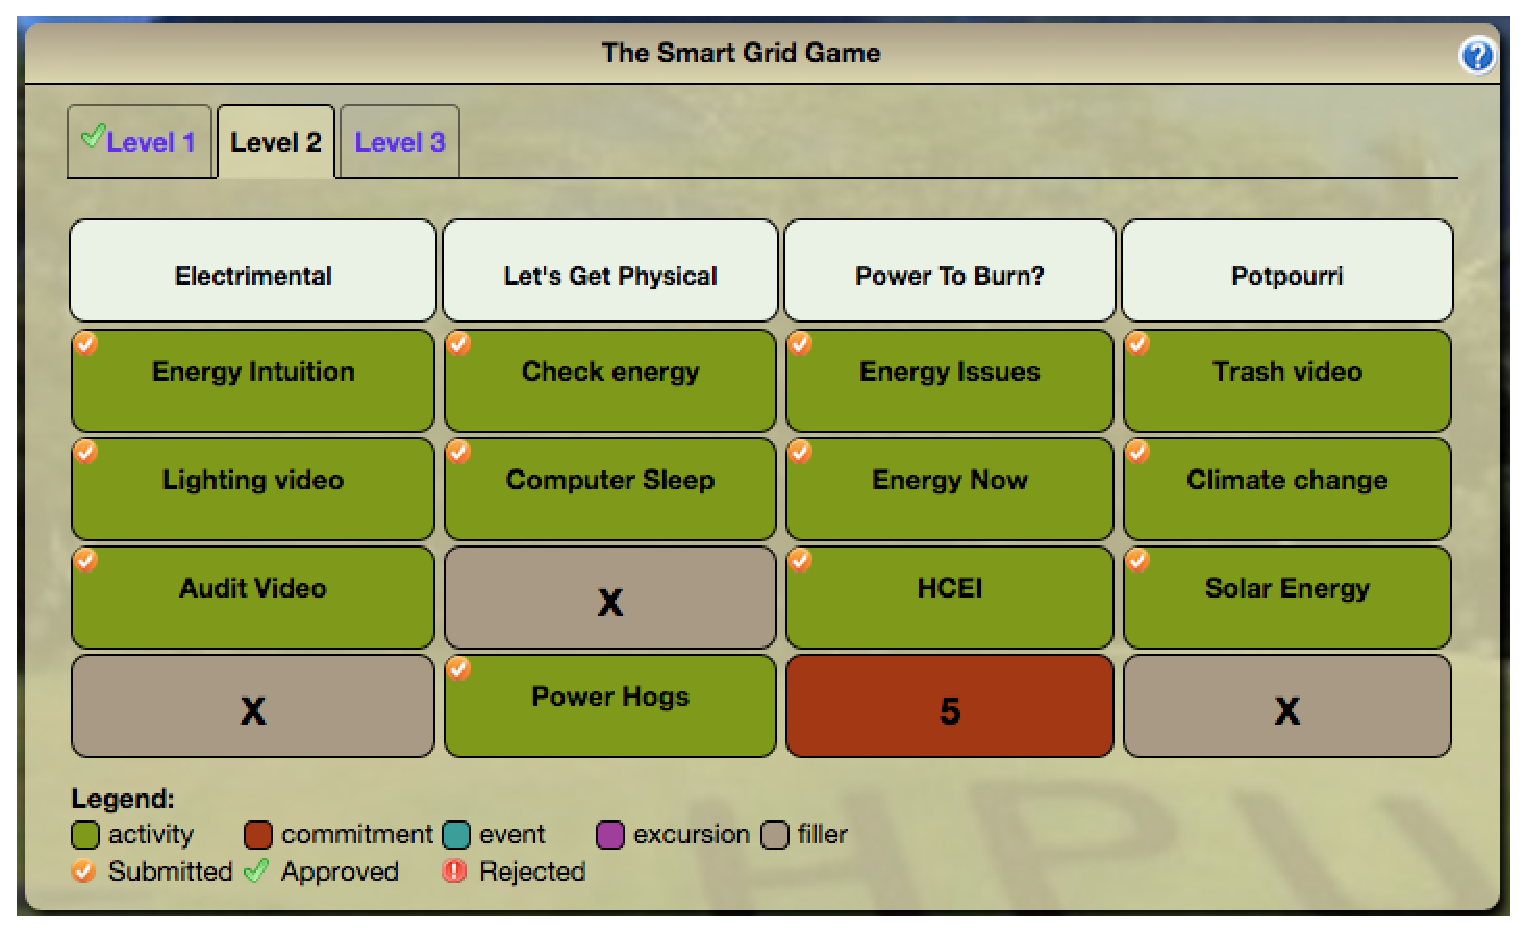
\includegraphics[height=2in,width=3.5in]{HPU-SGG-level2.eps}}
		\subfigure[HPU SmartGrid Game Level3]{\label{fig:hpu-level3}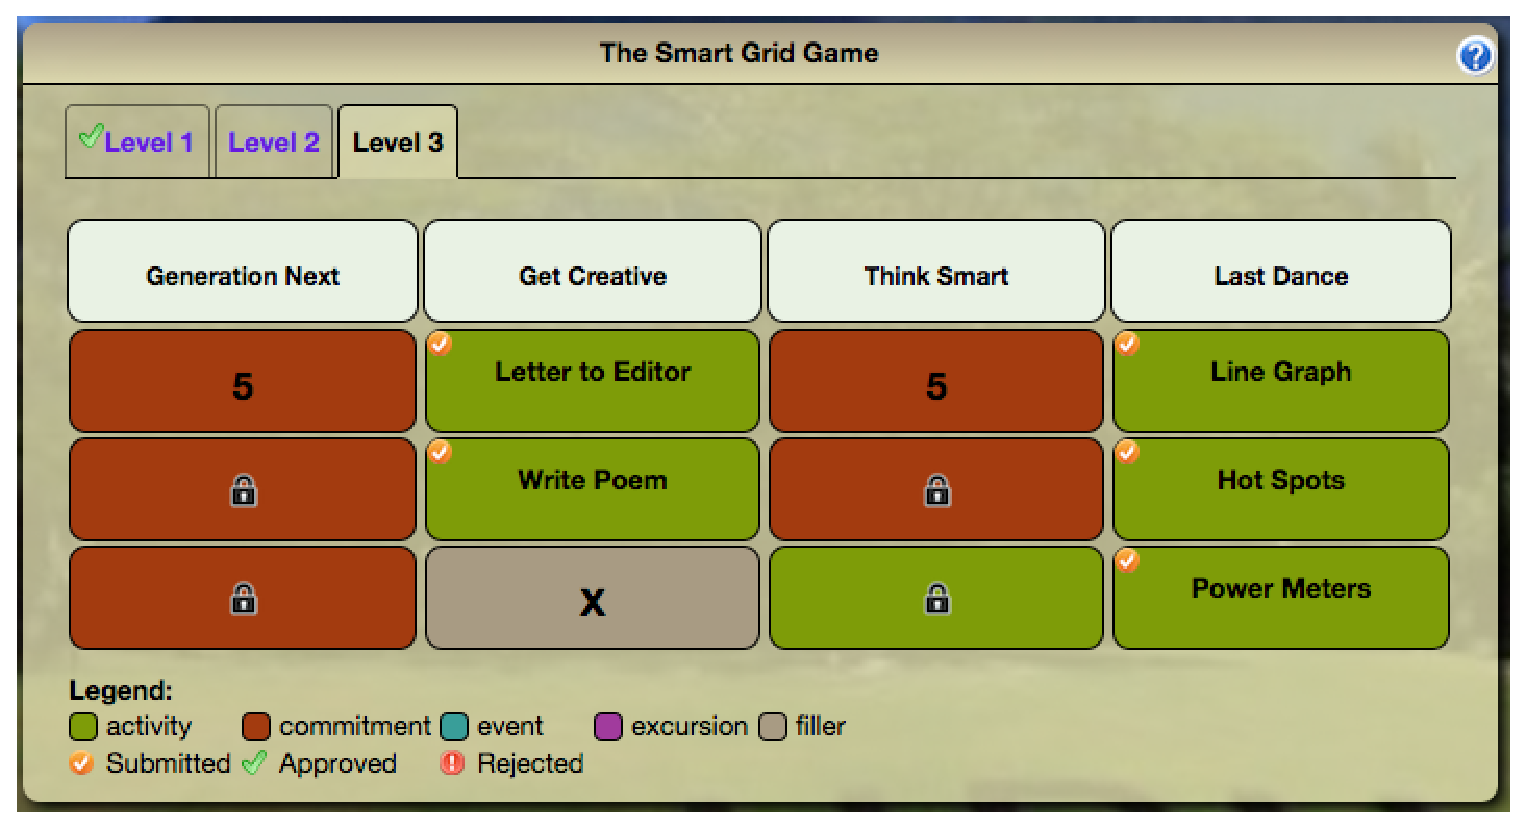
\includegraphics[height=2in,width=3.5in]{HPU-SGG-level3.eps}}
		\caption{HPU SmartGrid Game Layouts}
		\label{fig:HPU-SGG}
\end{figure}

\begin{figure}[htbp]
	\centering
		\subfigure[EWC SmartGrid Game Level1]{\label{fig:ewc-level1}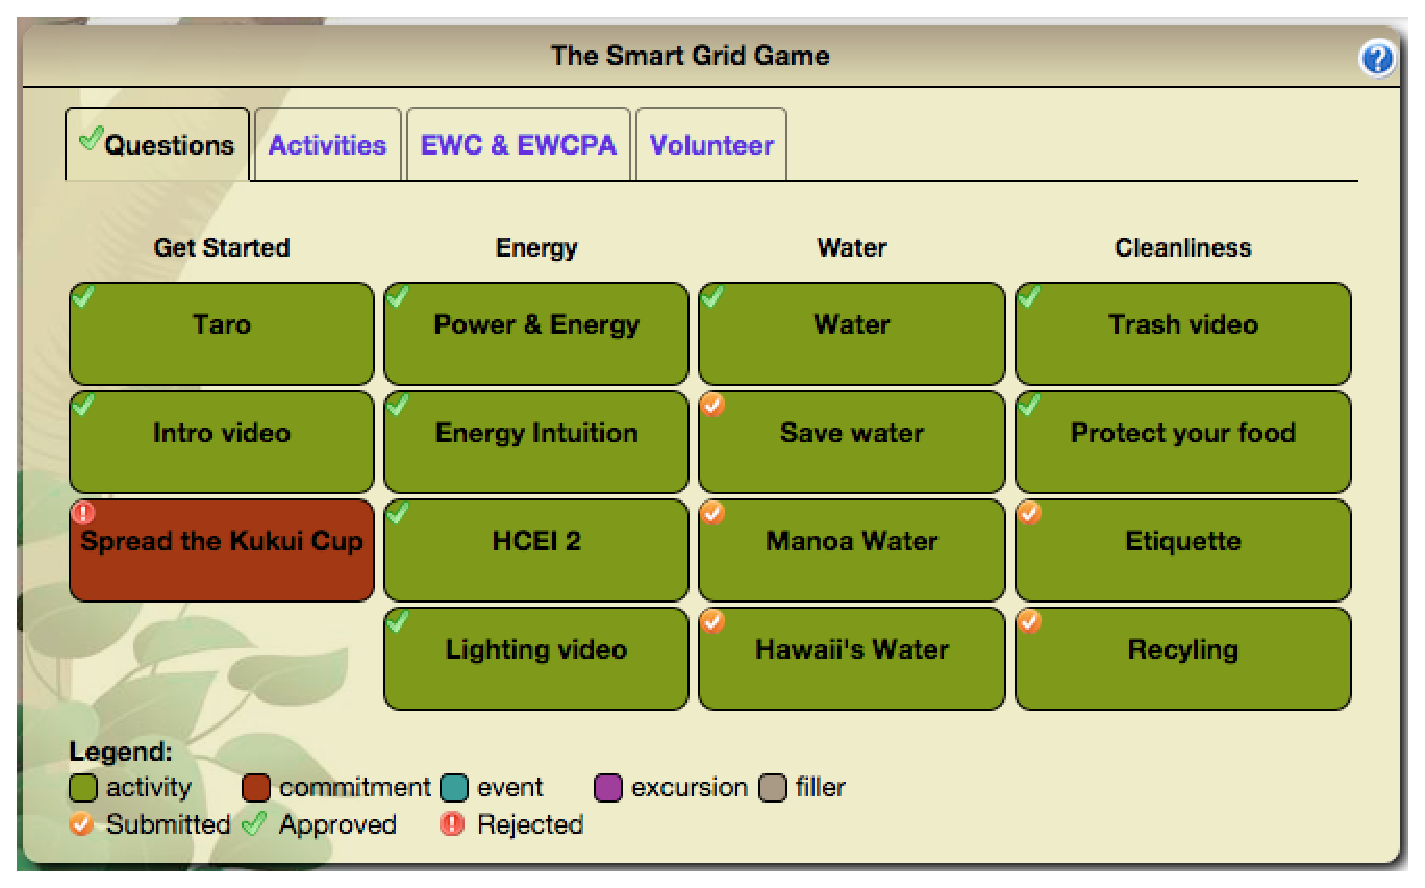
\includegraphics[height=1.7in,width=3.5in]{EWC-SGG-level1.eps}}
		\subfigure[EWC SmartGrid Game Level2]{\label{fig:ewc-level2}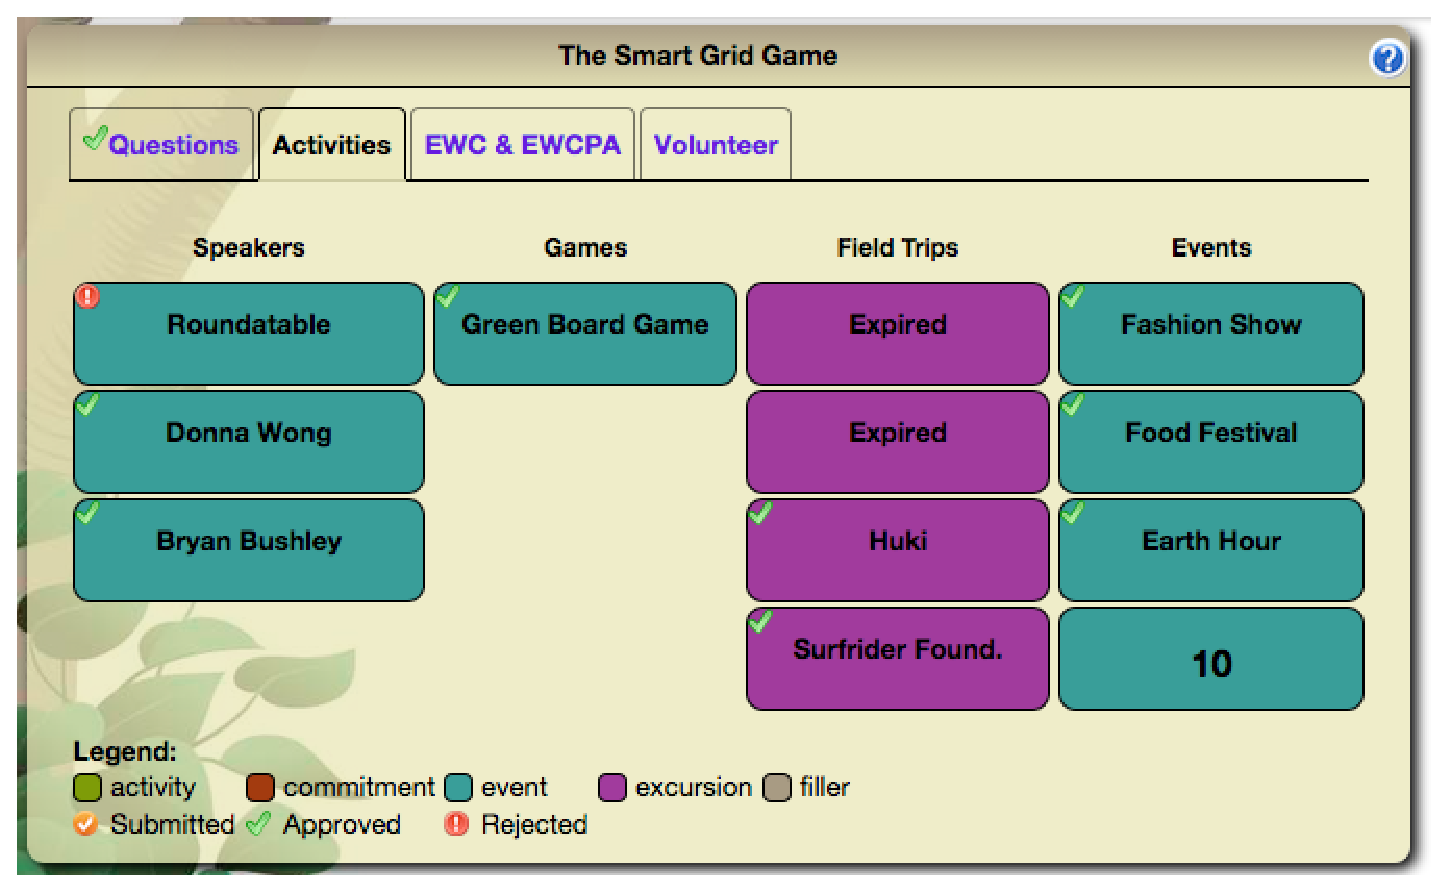
\includegraphics[height=1.7in,width=3.5in]{EWC-SGG-level2.eps}}
		\subfigure[EWC SmartGrid Game Level3]{\label{fig:ewc-level3}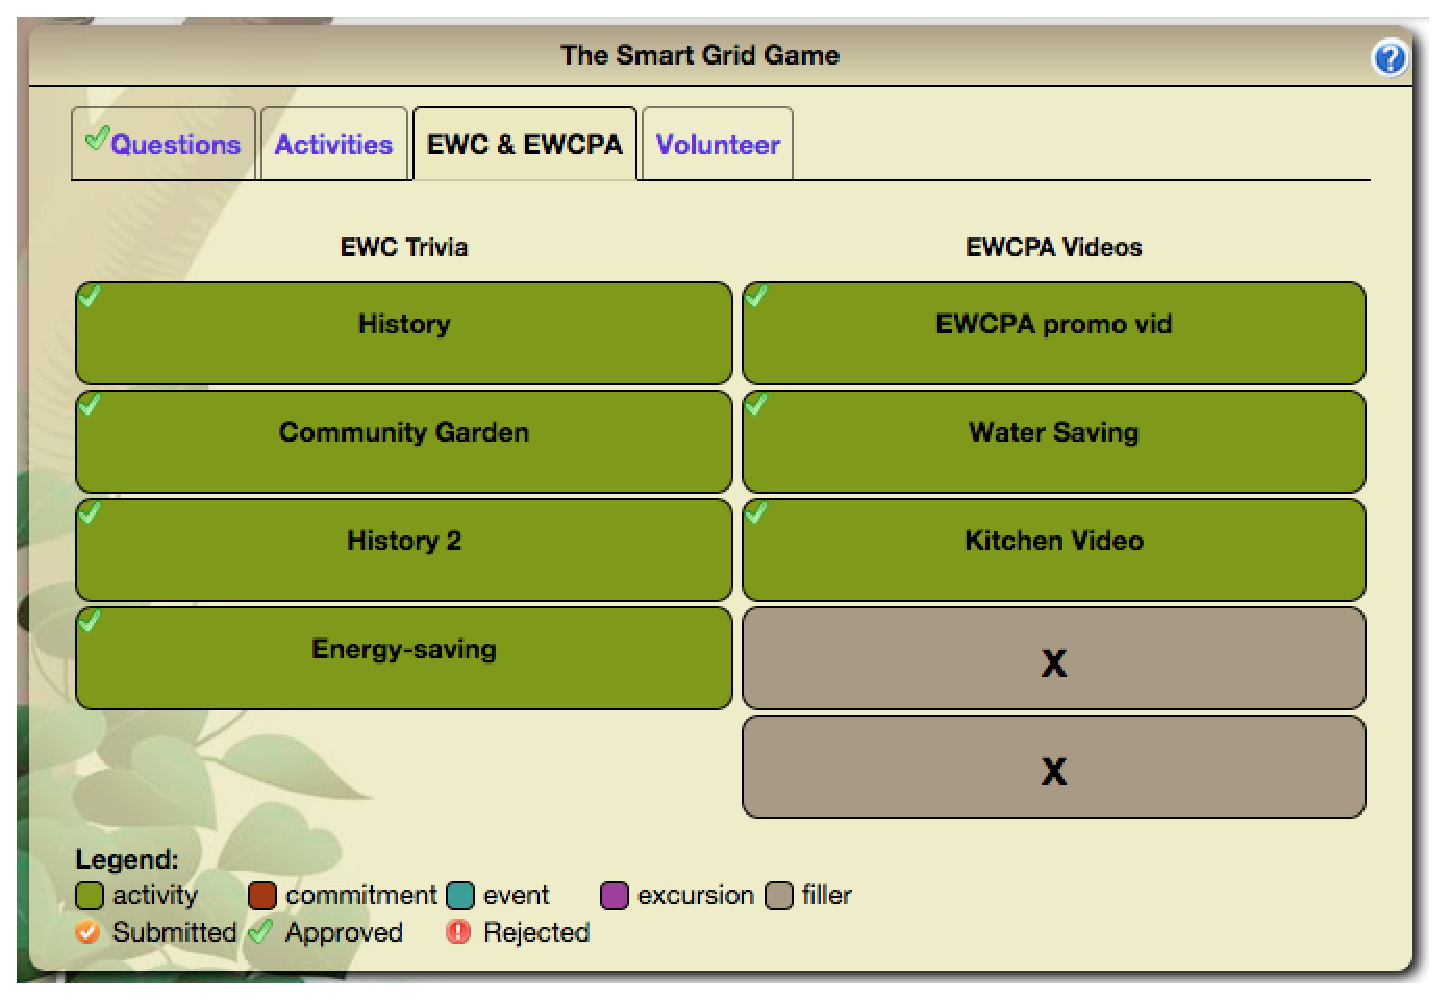
\includegraphics[height=1.7in,width=3.5in]{EWC-SGG-level3.eps}}
		\subfigure[EWC SmartGrid Game Level4]{\label{fig:ewc-level4}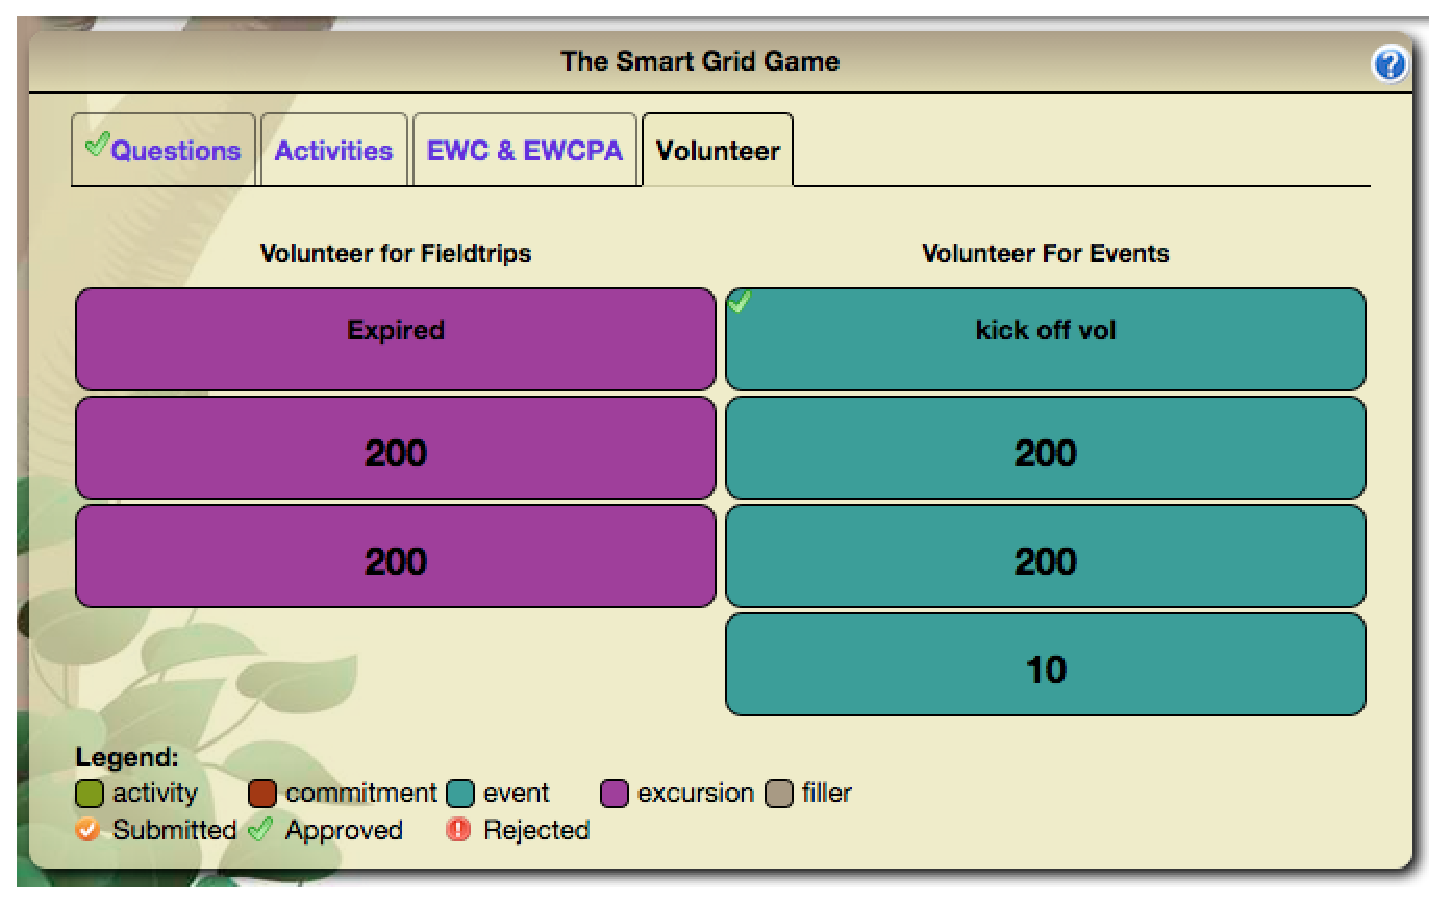
\includegraphics[height=1.7in,width=3.5in]{EWC-SGG-level4.eps}}
		\caption{EWC SmartGrid Game Layouts}
		\label{fig:EWC-SGG}
\end{figure}

\begin{figure}[htbp]
	\centering
		\subfigure[HNS SmartGrid Game Level1]{\label{fig:gs-level1}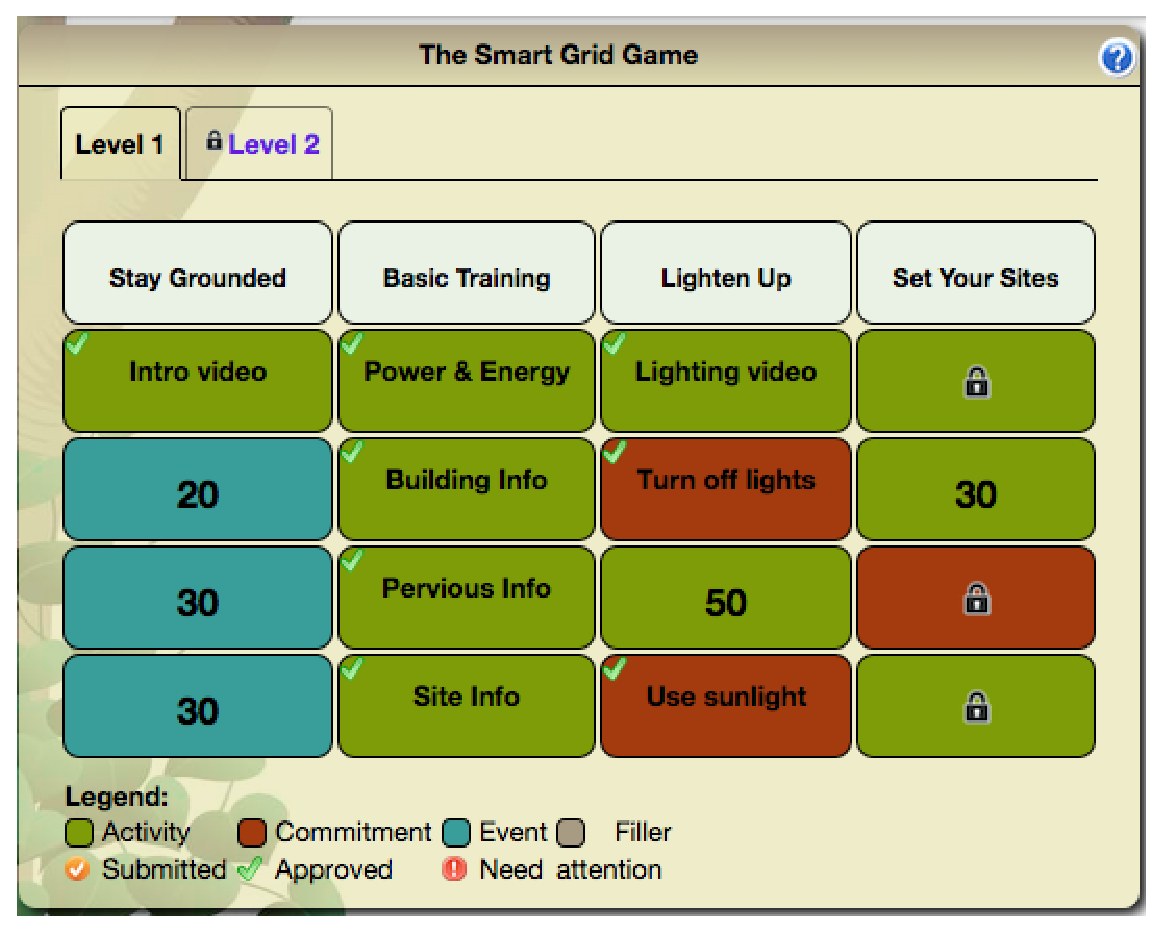
\includegraphics[height=2in,width=3.5in]{GS-SGG-level1.eps}}
		\subfigure[HNS SmartGrid Game Level2]{\label{fig:gs-level2}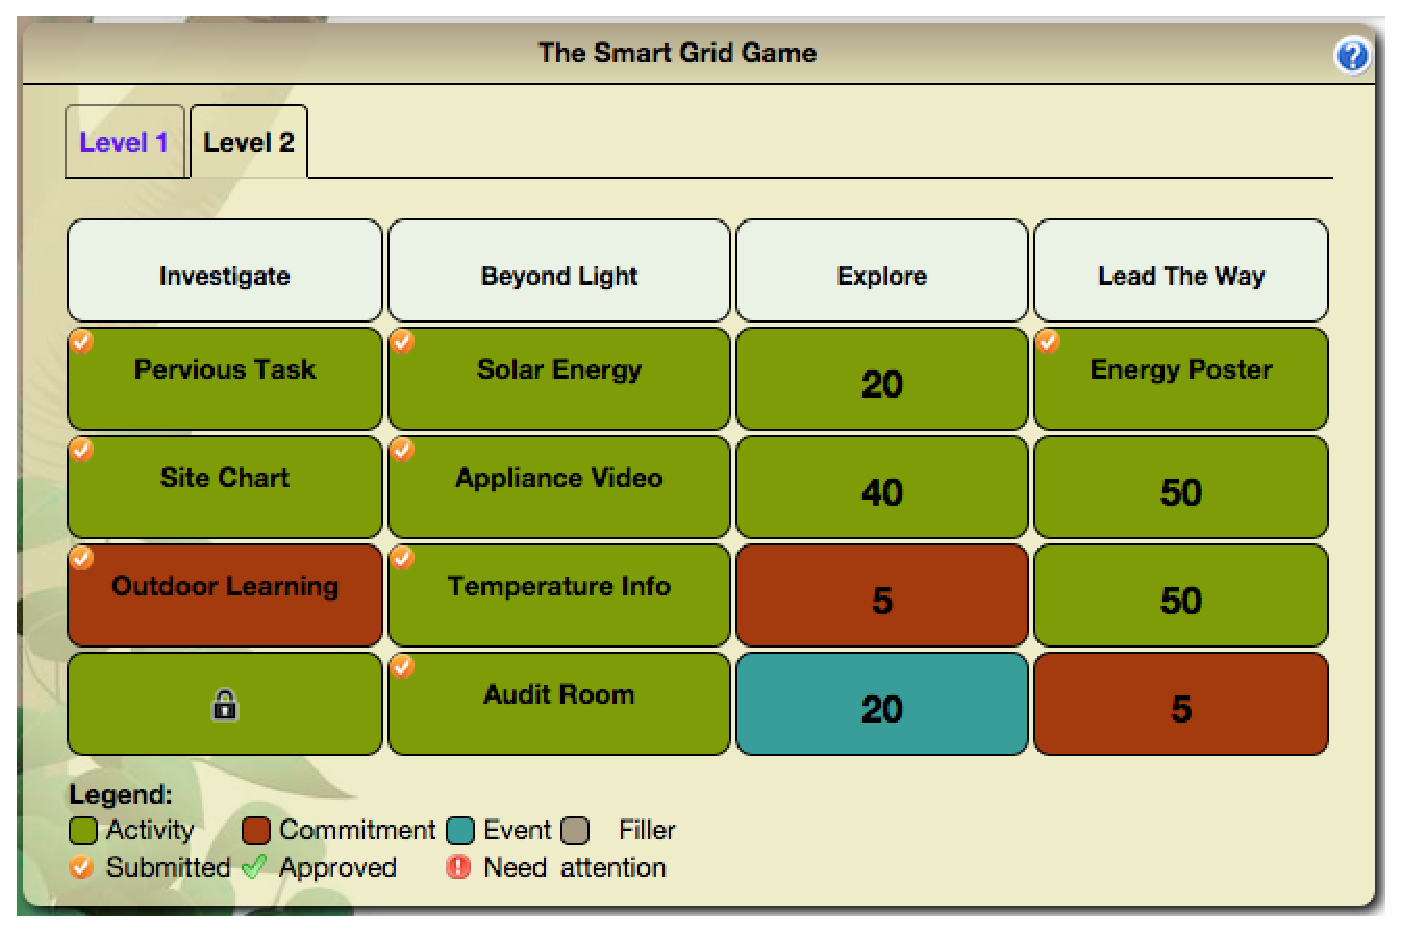
\includegraphics[height=2in,width=3.5in]{GS-SGG-level2.eps}}
		\caption{HNS SmartGrid Game Layouts}
		\label{fig:GS-SGG}
\end{figure}

\subsubsection{Branding Customization}
The look and feel of the challenges website are difference between the different organizations, which is customized using the customization feature of the Makahiki framework. The user interface was customized to ``brand'' each challenge. The list of customizable branding are:

\begin{itemize}
\item Logo
\item Site name
\item Challenge name
\item Team label
\item Landing page text
\item About page text
\item Sponsor text and logo
\item Theme
\end{itemize}

\subsubsection{System Configuration}

The system configuration includes the email server integration, authentication server integration, whether to use Facebook or not, and the smart meter connections. 

\autoref{table:system-configurations} lists the different configurations between the seven real world instances of Makahiki.

\begin{table}[ht!]
  \centering
  \begin{tabular} {|c|l|P{0.22\linewidth}|P{0.1\linewidth}|P{0.1\linewidth}|P{0.15\linewidth}|}
    \hline
    \tabhead{Instances} &
    \tabhead{Email server} &
    \tabhead{Authentication server} &
    \tabhead{Use Facebook} &
    \tabhead{Smart meters} & 
    \tabhead{Smart meter model} \\
    \hline
    UHM2011 & Gmail & UHM CAS & \checkmark & \checkmark & Shark\\
    \hline
    UHM2012 & Gmail & UHM CAS & \checkmark & \checkmark & Shark\\
    \hline
    UHM2014 & Gmail & UHM CAS & \checkmark & \checkmark & Shark\\
    \hline
    HPU2012 &  HPU email & HPU LDAP & \checkmark & \checkmark & eGauge\\
    \hline
    HPU2013 & HPU email & HPU LDAP & \checkmark & \checkmark & eGauge\\
    \hline
    EWC2012 & Gmail & UHM CAS\& Internal & \checkmark &   & \\
    \hline
    HNS2013 & Gmail & Internal &  &  & \\
    \hline
  \end{tabular}
  \caption{System Configuration Differences}
  \label{table:system-configurations}
\end{table}

In order to send emails to the players, Makahiki needs to be configured to use an email server to send the emails. In the UHM, EWC and HNS cases, the Gmail server was used to send out emails. In the HPU case, the system admin created a specific email account for the HPU Kukui cup (kukuicup@hpu.edu) in their existing email server, and configured Makahiki to use the HPU email server. 

The IT infrastructure at UH and HPU provided authentication services using CAS (Central Authentication Service) and LDAP, while EWC used the built-in Django authentication.  

Because the HNS instance was targeted for elementary school, Facebook integration was turned off in its configuration. In the other instances, Facebook integration was turned on and was used extensively during the game.

UH and HPU used different metering infrastructure, and EWC collected their resource data manually.  Since the EWC
residence halls did not have internet-enabled meters, resource consumption data had to be entered by
the game managers manually.

\subsection{Cloud Hosting Experiences}
\label{section:cloud-hosting}

Makahiki supports two types of hosting configurations. One is local hosting where the application runs on the organization's own IT infrastructure. The other is cloud hosting where the application runs on the Heroku's cloud infrastructure.

\autoref{table:hosting-configurations} lists the different hosting configurations between the seven real world instances of Makahiki. For the instances that hosted on the cloud infrastructure, the cloud service costs are also included in the table.  

\begin{table}[ht!]
  \centering
  \begin{tabular} {|c|c|c|c|c|}
    \hline
    \tabhead{Instances} &
    \tabhead{Hosting} &
    \tabhead{Other cloud services} &
    \tabhead{Duration} &
    \tabhead{Cloud service cost} \\
    \hline
    UHM2011 & Local Mac OS server & N/A & 3 weeks & N/A \\
    \hline
    UHM2012 & Heroku cloud & Amazon S3, Memcache & 9 months & \$908\\
    \hline
    UHM2014 & Heroku cloud & Amazon S3, Memcache & 2 weeks & \$150\\
    \hline
    HPU2012 &  Local CentOS server & N/A & 3 weeks & N/A\\
    \hline
    HPU2013 &  Local CentOS server & N/A & 3 weeks & N/A\\
    \hline
    EWC2012 & Heroku cloud & Amazon S3, Memcache & 2 weeks & \$9 \\
    \hline
    HNS2013 & Heroku cloud & Amazon S3, Memcache & 7 months & \$146 \\
    \hline
  \end{tabular}
  \caption{Hosting Configuration Differences}
  \label{table:hosting-configurations}
\end{table}

We installed Makahiki for the UHM 2011 instance locally in a Mac XServe server hosted in the Information and Computer Science department at the University of Hawaii at Manoa. We assisted the installation of the HPU instance by working with the system admin personnel at HPU. For the EWC, HNS and the 2012, 2014 UHM instances, we deployed and managed the instances in the Heroku cloud infrastructure.

Although there are some costs in the case of hosting the Makahiki games in the Heroku cloud infrastructure, there is no need for maintaining the local infrastructure, such as keeping the server running, upgrades, patching as well as locating physical space for the server. There is no need to allocate IT support staff resource to do the system admin. The long term cost of managing the local infrastructure is potentially higher. A serious game normally runs for a certain duration, so the organization only needs to pay for the charge for cloud infrastructure during that period.   

The following sections discuss the cloud services Makahiki used and its associated cost:

\subsubsection{Heroku Cloud Service: Dynos and Database}

One major benefit of using cloud infrastructure is the capability of dynamically adjust the computing resource for the application with scaling up when the usage demand is high and scaling down when the usage demand is low. This can be easily managed in the Heroku cloud infrastructure by the way of adjusting the numbers of Dyno and different type of database allocated to the application. Dynos are the units of computing power on Heroku, isolated containers that run the deployed application. Heroku provides different sizes (computing power) of Dynos and Postgres databases with different pricing \cite{heroku-pricing}. \autoref{table:cloud-configurations} lists the resource allocations to the real world instances of Makahiki in the Heroku cloud infrastructure. At the time of the hosting, there was only one size of dynos which was provisioned as 512MB RAM with 1xCPU Share. They were priced as \$34.50 per month, with the first dyno free of charge.

\begin{table}[ht!]
  \centering
  \begin{tabular} {|c|P{0.12\linewidth}|P{0.5\linewidth}|P{0.14\linewidth}|}
    \hline
    \tabhead{Instances} &
    \tabhead{Avg. Number of Dynos} &
    \tabhead{Database} &
    \tabhead{ Avg. Monthly Cost} \\
    \hline
    UHM2012 & 2.8 & Standard 0:  1 GB RAM, 64 GB storage, 120 connections (\$50/month) & \$100 \\
    \hline
    UHM2014 & 4 & Standard 2: 3.5 GB RAM, 256 GB storage, 400 connections (\$200/month) & \$300 \\
    \hline
    EWC2012 & 1 & Basic: 10 million rows limit (\$9/month) & \$10 \\
    \hline
    HNS2013 & 1.3 & Basic: 10 million rows limit (\$9/month) & \$20 \\
    \hline
  \end{tabular}
  \caption{Heroku Hosting Configuration}
  \label{table:cloud-configurations}
\end{table}

The UHM2014 instance had the highest monthly cost while the EWC2012 instance had the lowest monthly cost. The costs were corresponding to the use of the type of database and the number of dynos, which is based on the usage demand of the game instances. There were over 1,000 eligible registered players in the UHM instances, so higher provision was needed. Since EWC and HNS instances only has 130 users and 10 users respectively, a lower provision was sufficient. 

Before hosting the Makahiki instances on Heroku, we had to decide what are the appropriate provisions for these instances with acceptable run time performance. 
We did several performance tests with the Makahiki instance deployed on Heroku, and decided that 5 dynos was sufficient for servicing about 1,000 users in the first cloud instance, 2012 UHM Kukui Cup. We did not perform extensive performance testing, knowing that we can always adjust the allocation of dynos during the competition if we observe the dynos are over-loaded or under-utilized. The performance tests were performed using the Apache JMeter \cite{jmeter}. \autoref{fig:performance-test} shows the results of running the tests with 2 dynos against 100 concurrent users and 5 dynos against 250 concurrent users.

\begin{figure}[ht!]
	\centering
		\subfigure[2 dynos against 100 concurrent users]{\label{fig:2dynos}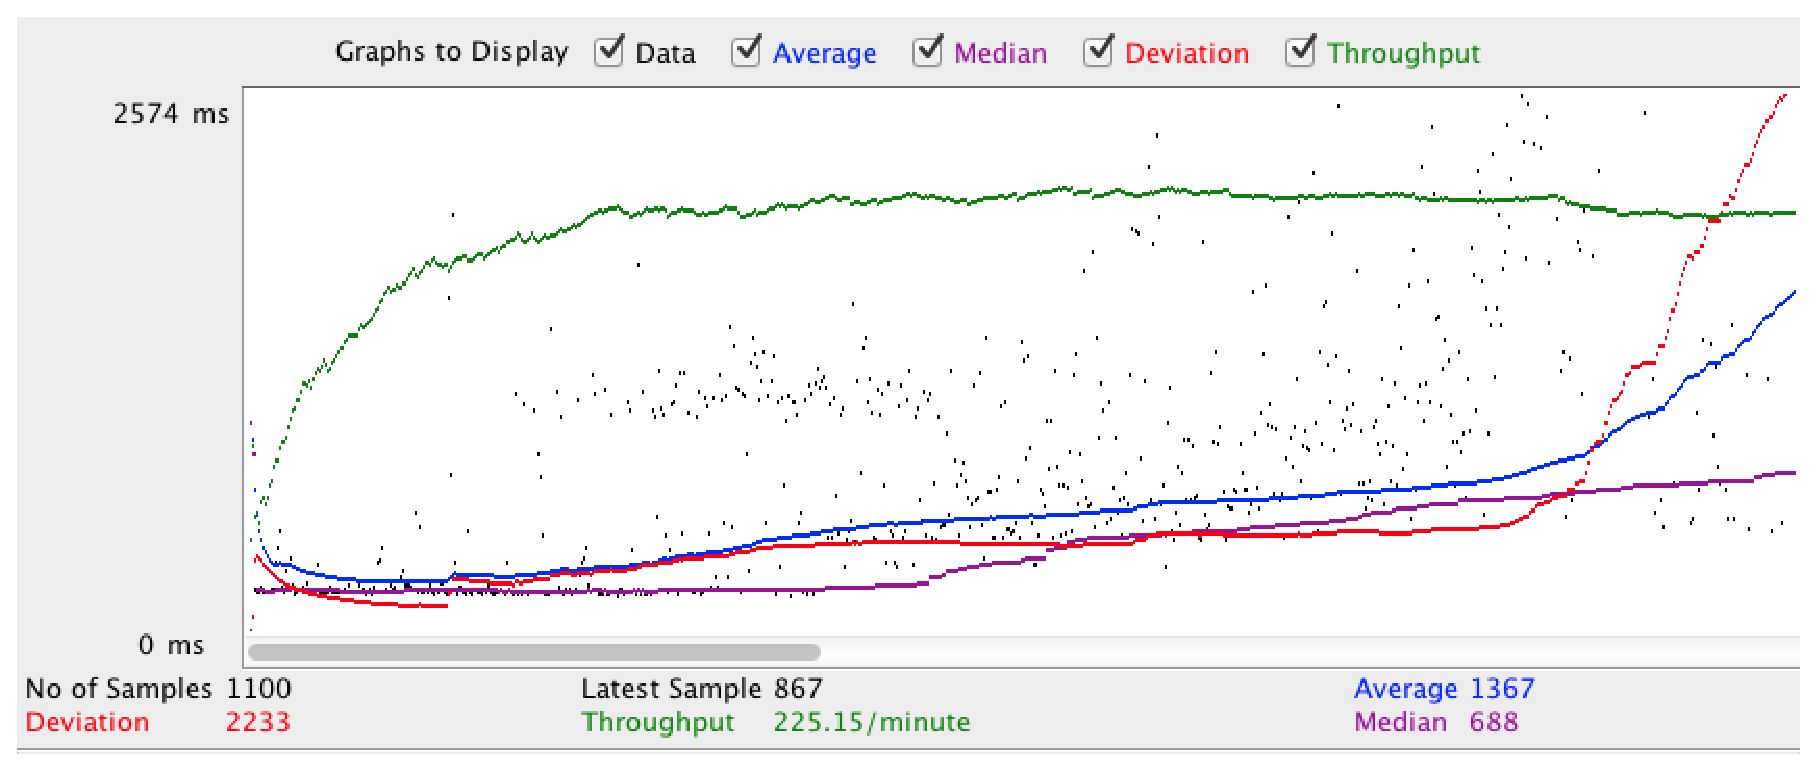
\includegraphics[height=2.2in]{2dynos100users}}
		\subfigure[5 dynos against 250 concurrent users]{\label{fig:5dynos}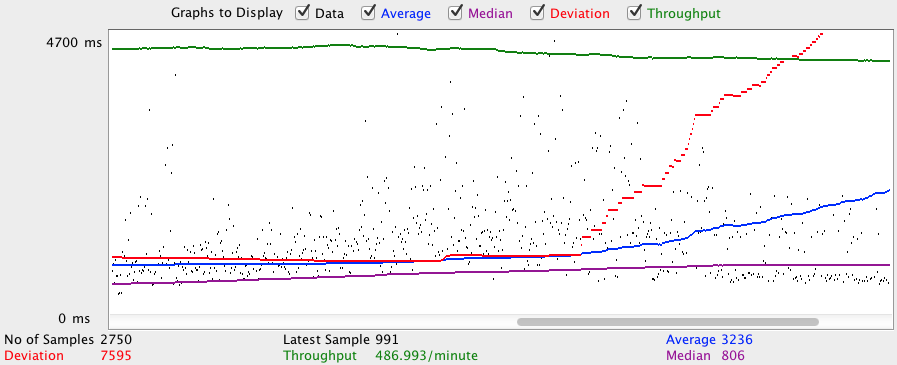
\includegraphics[height=2.2in]{5dynos250users}}
		\caption{Performance testing to determine the appropriate number of dynos}
		\label{fig:performance-test}
\end{figure}

We configured the Heroku cloud-based 2012 UHM instance to run with 5 dynos initially. After 5 days, we noticed that the dynos were under utilized, so we decreased the number of dynos to 4 and kept it run for about 1 month through the first 2 rounds. During the third round, the number of active players decreased, so we scaled down the Heroku dyno further to 2 dynos. At the beginning of the fourth round, we anticipated there may be a surge in website usage because of the new contents available in a new round, we scaled up the dynos to 4 again and found that after a while, the usage was down thus we scaled down the dynos to 2 and kept the game running to the end. \autoref{fig:dynamic-dynos} shows the dynamic dyno allocation during the UHM 2012 instance

\begin{figure}[ht!]
  \center
  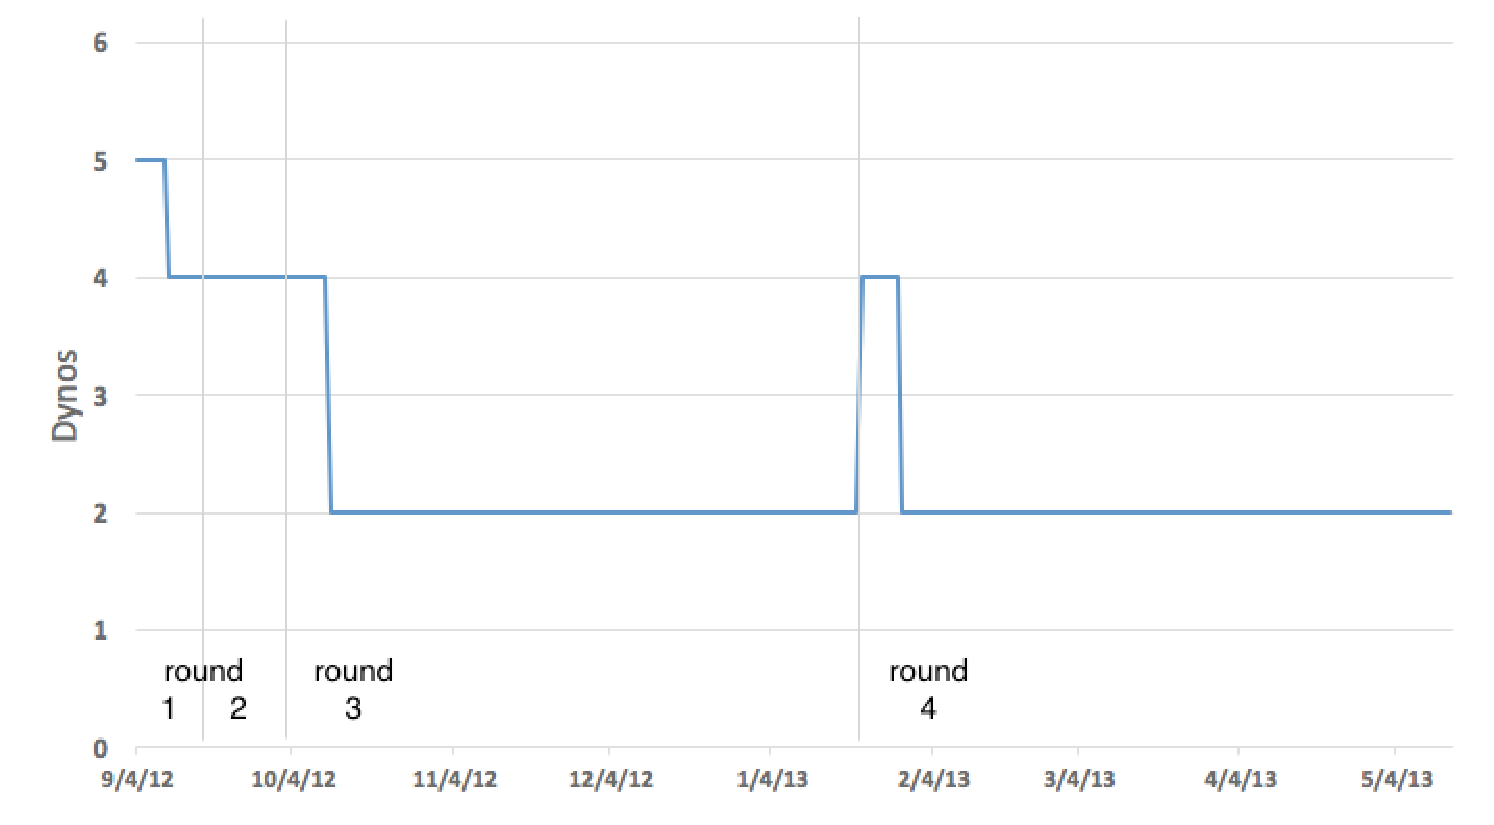
\includegraphics[width=0.9\columnwidth]{uhm2012-dynos}
  \caption{Dynamic Heroku dyno allocation during the UHM 2012 instance}
  \label{fig:dynamic-dynos}
\end{figure}

In the 2014 UHM instance, which was also deployed on the Heroku cloud infrastructure for the similar size of user base as in the 2012 Kukui Cup, 4 dynos were allocated for the entire duration of the 2 weeks competition because of its short term nature. We also performed a experiment to see if there is any performance difference when using the upgraded ``Standard 2'' cloud database. We did not observe any noticeable performance improvement with the upgraded but much more expensive database. We consider the ``Standard 0'' database would be sufficient to support the 2014 instance, thus bringing the cost for this kind of Makahiki instance to around \$100 per month.

In the case of EWC2012 and HNS2013 instances, because the user base is much smaller, about 130 and 10 users respectively, we used a less expensive ``Basic'' Heroku cloud database and allocated 1 dyno most of the time to achieve acceptable application performance. The two weeks EWC2012 competition found that the 1 dyno provisioned was sufficient without any performance complaints. The HNS2013 instance was initially provisioned with 1 dyno.  After three months, the game manager encountered occasional slow loading of the smart grid game page, so we increased the number of dynos to 2. Later on, we noticed the usage of the game site was low so we decreased the number of dynos back to 1 without affecting the running game. On average, the HNS instances use 1.3 dynos during the competition period. 

\subsubsection{Amazon S3 Cloud Service}

In additional to Heroku, Makahiki also integrates with other cloud services such as Amazon S3 \cite{amazons3}. During the deployment, Makahiki stores about 9 MB of static media files on Amazon S3. During the game, Makahiki uses S3 to store all the user uploaded medias such as player profile images, submission files, etc. Depending on the length of the game, number of players,  and the number of submission files, the usage of S3 storage might be different between various instances. \autoref{table:s3-usage} shows the Amazon S3 storage usage for the 4 real world Makahiki instances. According to S3 pricing \cite{amazons3}, the charge for the first 1 TB per month is \$0.03 per GB, and \$0.004 per 10,000 GET requests. With this very low cost of using S3, the cost of using S3 for real world Makahiki instances was negligible.

\begin{table}[ht!]
  \centering
  \begin{tabular} {|c|c|c|}
    \hline
    \tabhead{Instances} &
    \tabhead{Amazon S3 storage} &
    \tabhead{Cost} \\
    \hline
    UHM2012 & 204M & \$0.01 \\
    \hline
    UHM2014 & 101M & \$0.008 \\
    \hline
    EWC2012 & 11MB & \$0.004 \\
    \hline
    HNS2013 & 10MB & \$0.004 \\
    \hline
  \end{tabular}
  \caption{Amazon S3 storage usage for Makahiki instances}
  \label{table:s3-usage}
\end{table}

\subsubsection{Memcache Cloud Service}

Another cloud service that Makahiki used is the memcache service. Several memcache services are provided via Heroku add-ons to applications hosted on Heroku. By default, Makahiki used the free tier memcache add-on from one of the service providers called MemCachier\cite{memcachier}. 

MemCachier's free tier memory cache service is limited to 25MB. Depending on the size of memory cache used by the Makahiki instance, the organization could choose to use a different tier of cache service. In Makahiki, memory cache is mainly used to store  runtime system-wide information and game data from online active players. The data in the cache has a defined TTL (time to live) value so if the data is not being access after the TTL, it will be removed from the cache. In the cases of the 4 real world Makahiki instances, 25MB is enough for running the game.

MemCachier provides a simple usage page to monitor the cache usage for your application, as shown in \autoref{fig:memcachier}. We used this tool to identify the cache usage need for the Makahiki instance and monitor a running instance's usage.

\begin{figure}[ht!]
  \center
  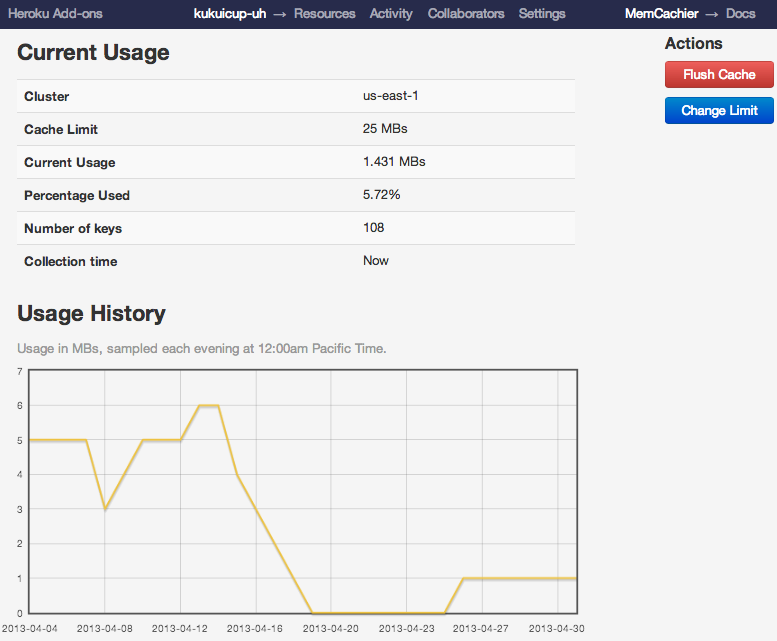
\includegraphics[width=0.8\columnwidth]{memcachier}
  \caption{Memory cache usage monitoring}
  \label{fig:memcachier}
\end{figure}

\subsubsection{Cloud Monitoring Service}

Makahiki uses a cloud application monitoring service called NewRelic to help monitor the game instances that are deployed to Heroku. The monitoring instrument is enabled by using the NewRelic client to start the Makahiki application. Once monitoring is enabled, the NewRelic service monitoring console shows runtime metrics of the Makahiki instance. \autoref{fig:newrelic-as} and \autoref{fig:newrelic-db} shows the monitoring screens for the application server metrics and database metrics respectively. Using this monitoring service, we can identify the performance issues from various sources of a running instance. It was also used to monitor the utilization of the allocated resources.

\begin{figure}[ht!]
  \center
  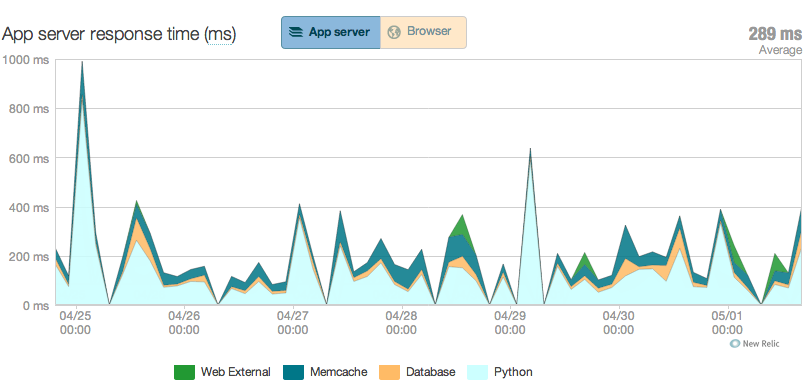
\includegraphics[width=0.9\columnwidth]{newrelic-as}
  \caption{NewRelic application monitoring}
  \label{fig:newrelic-as}
\end{figure}

\begin{figure}[ht!]
  \center
  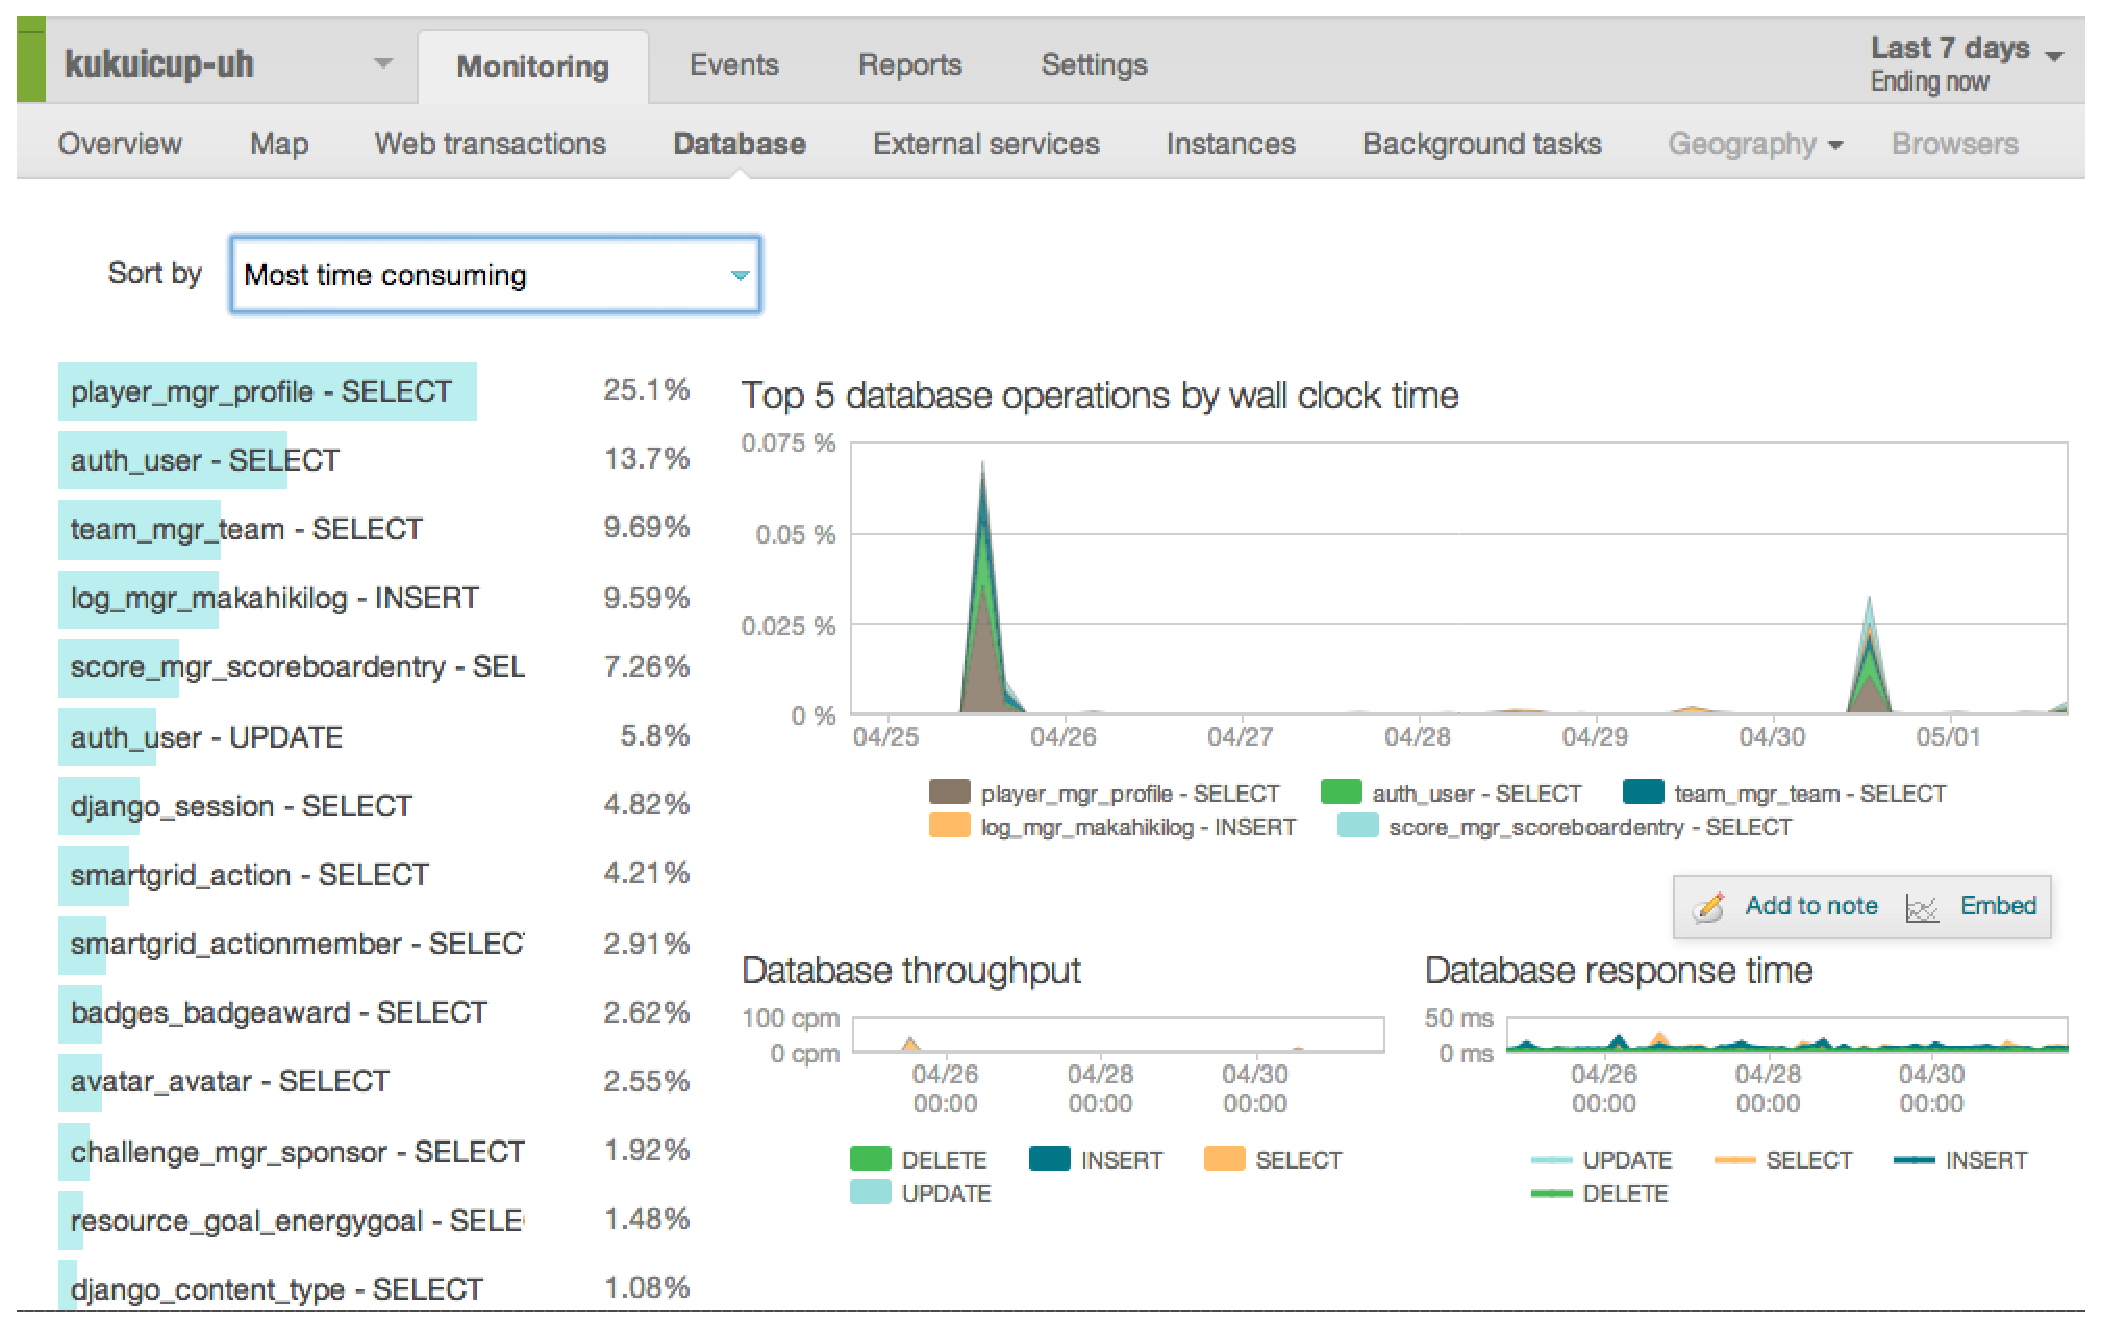
\includegraphics[width=0.9\columnwidth]{newrelic-db}
  \caption{NewRelic database monitoring}
  \label{fig:newrelic-db}
\end{figure}

In summary, this section described our experiences hosting the real world Makahiki instances in the Heroku cloud infrastructure. We compared the different resource provisions and associated costs for the different instances based on the number of players and the duration of the gams. Even during the game, the dynamic resource allocation capability of the cloud infrastructure provided a flexible and better utilization for this type of serious game. The areas we need to consider for the cloud infrastructure provisioning are:
\begin{itemize}
\item How many dynos / computing units to start with (for horizontal scaling)?
\item What kind of dynos, 1X or 2X (for vertical scaling)? 
\item How big / powerful / reliable should the database be? 
\item How much memory cache do we need?
\item What are the other cloud service (e.g, S3, monitoring) utilization?
\end{itemize}

\subsection{Summary}

This section described our experiences supporting seven real world Makahiki instances in four different organizations. The successful creation of these serious game instances provides evidence that Makahiki can be successfully tailored to the needs of different organizations. Among these instances, UHM and HPU used different metering infrastructure for energy data collection, EWC collected their resource data manually, and HNS did not have energy data at all. While UHM and HPU challenges involved only energy consumption data, the EWC challenge involved both energy and water consumption data. The IT infrastructure at UHM and HPU provided authentication services using CAS and LDAP, while EWC used both CAS and the built-in Django internal  authentication, and HNS used only the internal authentication. Moreover, the user interface was customized to ``brand'' each challenge with the logo, thematic elements, and the education content of the sponsoring organizations.

Lastly, the hosting infrastructure among these instances are different in two categories: local hosting for HPU and the 2011 UHM instances, and cloud hosting for EWC, HNS and 2012, 2014 UHM instances. These two types of hosting requirements created unique challenges for Makahiki. There are different costs associated with these hosting solutions. Although there are some incurred costs in the case of hosting the Makahiki games in the Heroku cloud infrastructure, there is no need for maintaining local infrastructure, such as keeping the server running, upgrades, patching as well as locating physical space for the server. There is no need to allocate IT support staff resource to do system admin. In addition, the dynamic resource allocation capability of the cloud infrastructure provides a flexible and efficient utilization of infrastructure resources in running the competition, especially in the case of short competition duration and varying user demands during the game.

\section{SGSEAM Assessment Results}
\label{sec:assessment-result}

This section describes the result of applying the formal assessment method of SGSEAM to the Makahiki framework to assess the strengths and weaknesses of the Makahiki as a serious game framework.

The SGSEAM assessment plan for Makahiki (\autoref{app:makahiki-assessment-plan}) describes two categories of assessment approaches. The {\em in-vivo} approaches of pre-post effectiveness study, in-game surveys, and post-hoc interviews were applied to the real-world UHM, HPU and EWC Makahiki instances. The other {\em in-vitro} approaches were applied to the UHM ICS691 serious game course as an in-lab experiment.  \autoref{fig:assessment-overview} provides the overview of assessment and participants for each SGSEAM stakeholders of the Makahiki framework. 

\begin{table}[ht!]
  \centering
  \begin{tabular}{|p{0.18\columnwidth}|p{0.35\columnwidth}|p{0.35\columnwidth}|}
    \hline
    \tabhead{Stakeholder} &
    \tabhead{Assessment Approach} &
    \tabhead{Participants}  \\
    \hline
    \multirow{4}{*}{Players} & Pre-Post effectiveness study & \multirow{4}{*}{UHM Kukui Cup players} \\
    \cline{2-2}
     & Self-reported effectiveness survey &  \\
    \cline{2-2}    
     & Self-reported usability survey &  \\
    \cline{2-2}
     & Engagement metrics &  \\
    \hline
   \multirow{2}{*}{System admins} & In-lab installation study & UHM ICS691 students \\
    \cline{2-3}
     & Post-hoc system admin interview & HPU Kukui Cup sysadmin \\
    \hline
   \multirow{2}{*}{Game designers} & In-lab game design study & ICS691 students\\
    \cline{2-3}
     & Post-hoc game designer interview & HPU \& EWC Kukui Cup game designers \\
    \hline
  Game managers & Post-hoc game manager interview & HPU \& EWC Kukui Cup game managers \\
    \hline
   Developers & In-lab game development study & ICS691 students\\
    \hline
  \end{tabular}
  \caption{SGSEAM assessments for Makahiki}
  \label{fig:assessment-overview}
\end{table}

As the assessment approaches were carried out, the assessment data were collected and stored in the data repository (\autoref{app:makahiki-data-repository}). The following sections describe the data analysis and the results for the assessment of each stakeholder.

\subsection{Makahiki Player Assessment}

We used four approaches to assess the player experience for the Makahiki framework. They are a pre-post effectiveness study, a self-reported effectiveness survey, a self-report usability survey, and engagement metrics. The real world Makahiki instances of the UHM Kukui Cup challenge were used for the Makahiki player assessments. 

\subsubsection{Pre Post effectiveness study}
\label{sec:player-pre-post-effectiveness-result}

In the 2011 Kukui Cup Challenge at the University of Hawaii at Manoa, there were over 1000 eligible players, who were mostly first
year college students living in the 5 residence halls. The challenge was designed to last for 3 weeks and the student players were divided into 20 teams based on the dorm locations where they resided. Each team's energy consumption was measured by a smart meter installed in various locations inside the resident hall. Makahiki recorded the energy consumption for the players before, during and after the challenge. Makahiki also recorded detailed logging data from every interaction between the players and the website. 

To assess the effectiveness of the framework for designing games that improve player literacy in sustainability, 
 two energy literacy surveys were conducted, one before the challenge (pre-game) and one after
the challenge (post-game). 

Robert Brewer designed and conducted the survey. The results are reported in his dissertation \cite{csdl2-10-08}. 24 players completed both surveys. Out of the total 19 energy literacy questions, the average number of questions answered correctly is 7.54 before the
challenge, and 8.96 after the challenge. This result indicates an 18\% (p=0.056) improvement on the
energy literacy.  Non-players as a control condition were also surveyed and found that their literacy did not change. The result is shown in the \autoref{fig:UHM-literacy-result}. According to Brewer \cite{csdl2-10-08}, ``Based on the questionnaire results, it appears that the energy knowledge of challenge participants increased modestly compared to those that did not participate in the challenge.''
\begin{figure}[ht!]
  \center
  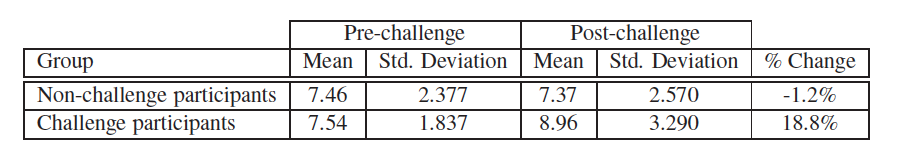
\includegraphics[width=0.9\columnwidth]{UHM-literacy-result}
  \caption{Literacy survey result from Brewer 's dissertation \cite{csdl2-10-08}}
  \label{fig:UHM-literacy-result}
\end{figure}

To assess the effectiveness of the framework for designing games that reduce players' resource consumption, The energy usage data that was collected before, during and after the
challenge were used to compare the differences.  Before the challenge, an energy usage baseline was established. 

Robert Brewer calculated the energy consumption data before and after the UHM 2011 Kukui Cup challenge. According to his dissertation \cite{csdl2-10-08}, 12 out of the total 20 teams reduced their energy
consumption compared to the baseline. The highest reduction was 16.1\%. However, 3 teams actually increased
their energy consumption, with the highest increase of 11.7\%. The result is shown in the \autoref{fig:UHM-energy-result}. Overall, the average reduction of the 20 teams was low (1.9\%).  According to Hodge's North America collegiate energy competition survey \cite{Hodge2010}, the average reduction in electricity use for these competitions is 9\%. This study did not provide strong evidence that the challenge results in effective reduction of energy use.

\begin{figure}[ht!]
  \center
  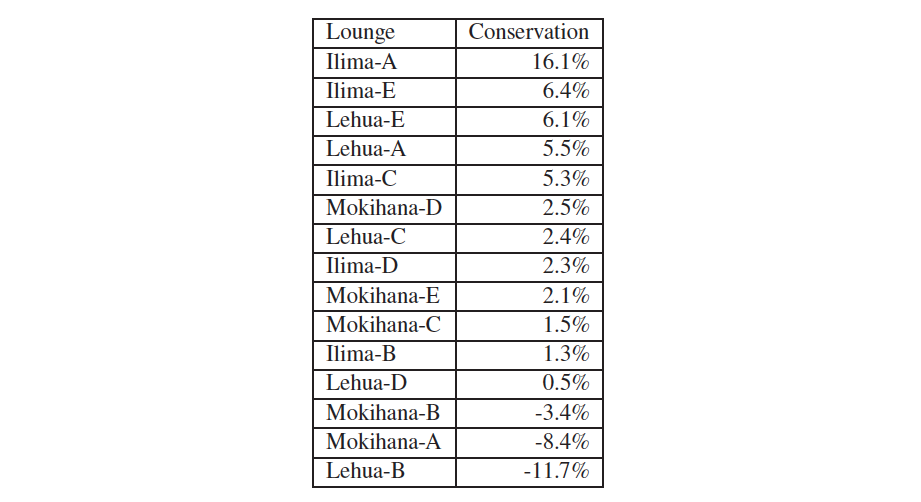
\includegraphics[width=0.9\columnwidth]{UHM-energy-result}
  \caption{Energy consumption result from Brewer's dissertation \cite{csdl2-10-08}}
  \label{fig:UHM-energy-result}
\end{figure}

In summary, this study indicates that Makahiki was successful in achieving player literacy improvement. It did not provide strong evidence that the challenge results in effective reduction of energy consumption by players. 

\subsubsection{Self-reported effectiveness survey}
\label{sec:player-self-reported-effectiveness-result}

A survey to gather the opinions of participants regarding the effect of the challenge to their sustainability awareness and behavior changes was included during the last round of the challenge. 
Two survey questions were used to assess the self-reported perception of the players regarding their interests in energy conservation and sustainability prior and after playing the Kukui Cup. 

In the 2011 UHM Kukui Cup challenge, 43 players completed the survey. The responses to the survey were provided in free text. We analyzed the free text responses and coded them into three categories: ``Yes'', ``No'', and ``Somewhat''. \autoref{table:interests-in-sustainability} lists results of the responses. \autoref{fig:effect-prior-after} illustrates the percentages of self-reported interests in the sustainability prior to the KuKui Cup and the effect after playing the Kukui Cup.

\begin{table}[ht!]
  \centering
  \begin{tabular} {|p{0.6\linewidth}|c|c|c|}
    \hline
    \tabhead{\multirow{2}{*}{Question}} & \multicolumn{3}{c|}{\tabhead{Number of Responses}} \\
    \cline{2-4}
    \tabhead{} & \tabhead{Yes} & \tabhead{No } & \tabhead{Somewhat}\\
    \hline
    Prior to playing the Kukui Cup, were you interested in energy conservation? & 24 & 8 & 11\\
    \hline
    Has the Kukui Cup increased your interest in energy conservation and sustainability?& 37 & 0 & 6 \\
    \hline
  \end{tabular}
  \caption{Interests in sustainability prior and after the KC (2011 UHM, n=43)}
  \label{table:interests-in-sustainability}
\end{table}

\begin{figure}[htbp]
	\centering
		\subfigure[interests in sustainability prior]{\label{fig:effect-prior}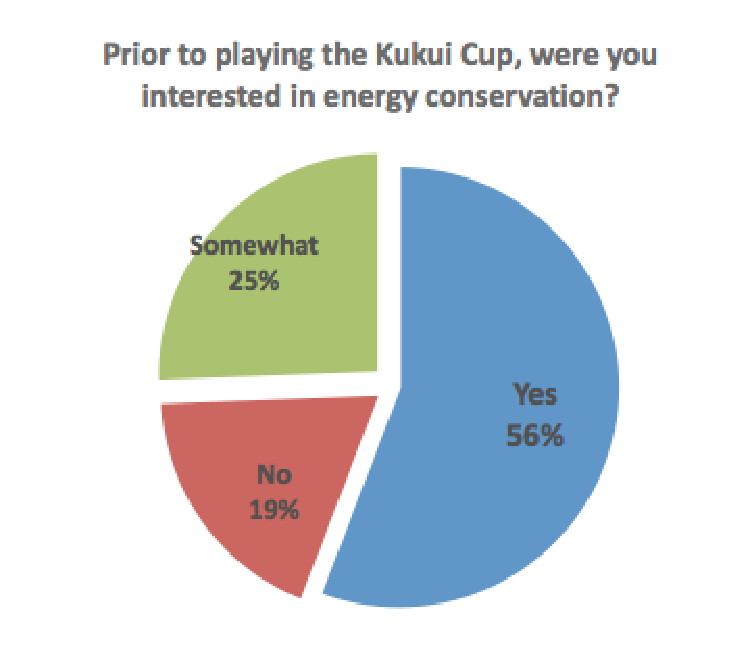
\includegraphics[height=2.2in]{effect-prior.eps}}
		\subfigure[increased interests in sustainability after]{\label{fig:effect-after}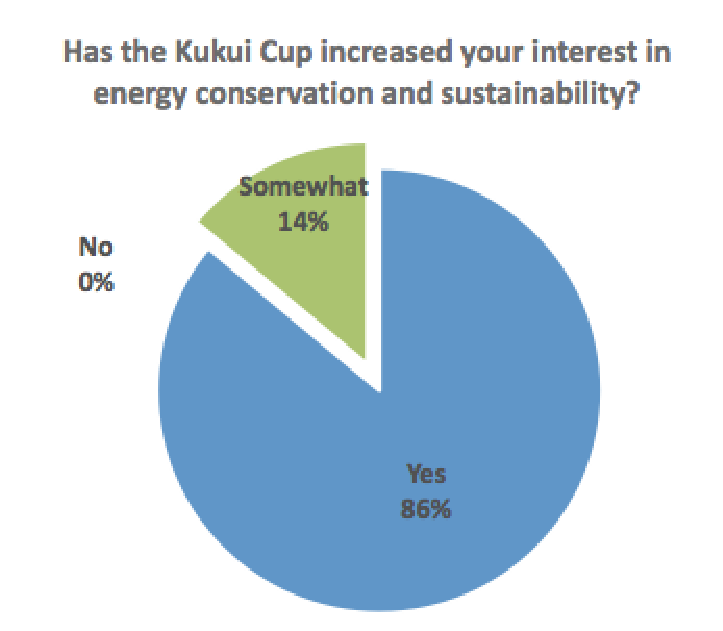
\includegraphics[height=2.2in]{effect-after.eps}}
		\caption{Interests in sustainability prior and after the UHM 2011 KC}
		\label{fig:effect-prior-after}
\end{figure}

The self-reported responses indicates that there are 19\% players who were not interested in the sustainability prior to the Kukui Cup. After playing the Kukui Cup, 100\% of responses reported an affirmative or somewhat affirmative increase of interests in sustainability. 

In 2012 UHM Kukui Cup challenge, the similar survey questions were included the last round. 44 players completed both the two questions. \autoref{table:interests-in-sustainability-2012} lists results of the responses. \autoref{fig:effect-prior-after-2012} illustrates the percentages of self-reported interests.

\begin{table}[ht!]
  \centering
  \begin{tabular} {|p{0.6\linewidth}|c|c|c|}
    \hline
    \tabhead{\multirow{2}{*}{Question}} & \multicolumn{3}{c|}{\tabhead{Number of Responses}} \\
    \cline{2-4}
    \tabhead{} & \tabhead{Yes} & \tabhead{No } & \tabhead{Somewhat}\\
    \hline
    Prior to playing the Kukui Cup, were you interested in energy conservation? & 28 & 4 & 12\\
    \hline
    Has the Kukui Cup increased your interest in energy conservation and sustainability?& 37 & 5 & 2 \\
    \hline
  \end{tabular}
  \caption{Interests in sustainability prior and after the KC (2012 UHM, n=44)}
  \label{table:interests-in-sustainability-2012}
\end{table}

\begin{figure}[htbp]
	\centering
		\subfigure[interests in sustainability prior]{\label{fig:effect-prior-2012}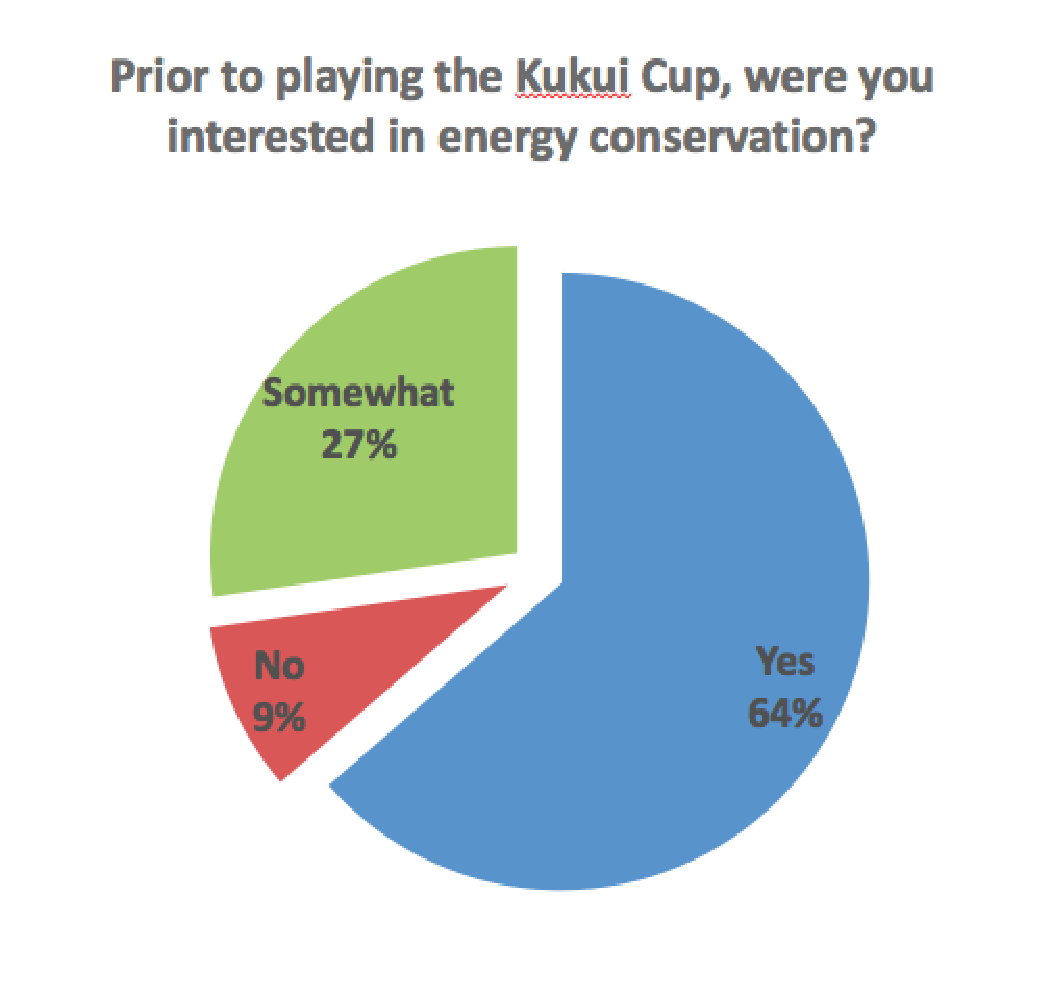
\includegraphics[height=2.2in]{effect-prior-2012.eps}}
		\subfigure[increased interests in sustainability after]{\label{fig:effect-after-2012}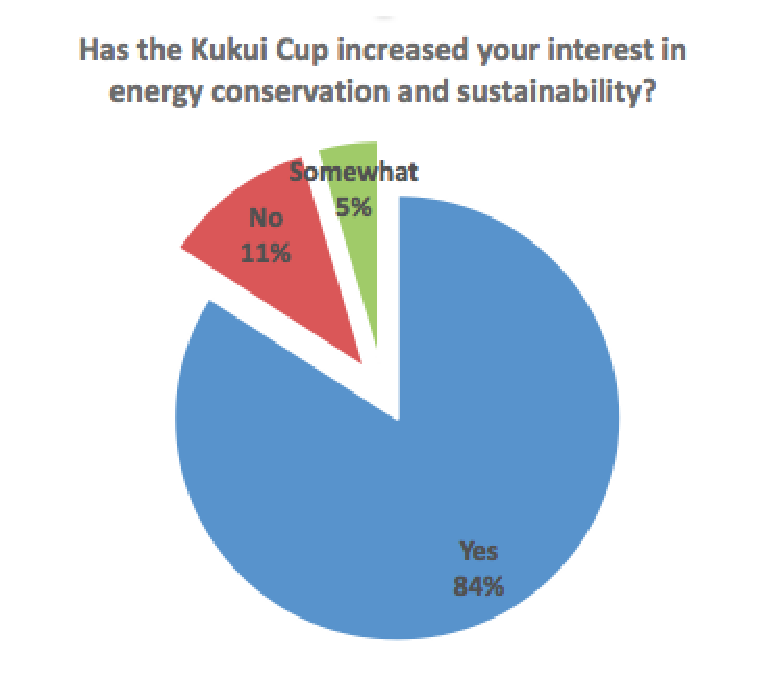
\includegraphics[height=2.2in]{effect-after-2012.eps}}
		\caption{Interests in sustainability prior and after the 2012 UHM KC}
		\label{fig:effect-prior-after-2012}
\end{figure}

The self-reported responses from 2012 KC indicates that there are a smaller percentage (9\%) of players than 2011 KC (19\%) that were not interested in the sustainability prior to the Kukui Cup. This could be due to the increasing sustainability exposure over years to the young students.  After playing the Kukui Cup, 89\% of responses reported an affirmative or somewhat increase of interests in sustainability. There are 5 players (11\%)  reported no changes of interests in sustainability. A closer look at the data indicates that the 5 players that reported no changes of interests also answered ``Yes'' or ``Somewhat'' interested to the sustainability prior to the Kukui Cup. The 4 players that reported no interests in sustainability also reported that playing KC had increased their interests.

\autoref{fig:sustainability-interests-samples} shows some sample responses from the students who considered the Kukui Cup had increased their interests in sustainability:
 
 \begin{figure}[ht!]
\begin{mybox}
\begin{compactenum}
	\item ``Yes. I'm more aware of everything I am using.''
	\item ``I've been interested, but the Kukui Cup has expanded and broadened my mind on what else I can be doing to help with conservation and sustainability. I think people are genuinely concerned, they just don't know how to exactly conduct them, or what other ways they can do it.''
	\item ``Yes, it made me realize that you can save a lot of money by turning off and unplugging a few things. (Hopefully lower tuition? =D )''
	\item ``It has increased my interest since I didn't know much about how much energy were using.''
	\item ``Some workshops made me think differently of how I use energy. Makes alternatives more interesting for me.''
	\item ``It taught me some new interesting facts about renewable energy and made me more aware.''	
\end{compactenum}
\end{mybox}
\caption{Sample responses of reported increased interests in sustainability}
\label{fig:sustainability-interests-samples}  
\end{figure}

There was a question in the 2011 KC survey asking about the players' perception about how would they describe the Kukui Cup. The players were asked to check all that applies to their agreement to the following descriptions of the Kukui Cup: ``Educational'', ``Fun'', ``Addictive'', ``So-so'', ``Difficult'', ``Boring'', ``Not useful'', and ``Other'' where they will type in their free text responses. There were 43 responses from the 2011 KC survey. The numbers of responses and their percentages are listed in  \autoref{table:how-is-kc} (sorted by percentage in descending order).

\begin{table}[ht!]
  \centering
  \begin{tabular} {|c|c|c|}
    \hline
    \tabhead{Question: How would you describe the Kukui Cup?} & \tabhead{Number of Responses} & \tabhead{Percentage}\\
    \hline
Educational	& 41 & 95\%\\
    \hline
Fun	& 39 & 91\% \\
    \hline
Addictive	 &19 & 44\%\\
    \hline 
So-so	& 9 & 21\%\\
    \hline
Other & 5 & 12\%\\   
    \hline 
Difficult	& 3 & 7\%\\
    \hline
Boring	& 1 & 2\%\\
    \hline
Not useful	& 0 & 0\\
    \hline
  \end{tabular}
  \caption{Self-reported Perception of the Kukui Cup in 2011 UHM KC (n=43)}
  \label{table:how-is-kc}
\end{table}
	
The majority of the responses indicated the players perceived the Kukui Cup as ``Educational'' (95\%) and ``Fun'' (91\%). 44\% of players perceived Kukui Cup as ``Addictive". On the other hand, 1 player (2\%) considered the Kukui Cup as ``Boring". The ``Other'' responses are: ``AWSOME-NESS''(1), ``engaging''(1), ``fun competition''(1), ``Great way to bond with others''(1), ``impressive''(1).

Another survey question was asked about the players' self reported behavior change during the challenge in the 2012 UHM Kukui Cup. The question is ``Did you change your behavior during the competition based on the commitment(s) you made? if so, how?" It is a free response question. 45 players completed the survey. The free text responses were categorized into three categories: ``Yes'', `already a habit'', and ``no''. The results are listed in \autoref{table:behavior-change}.

\begin{table}[ht!]
  \centering
  \begin{tabular} {|p{0.5\linewidth}|c|c|}
    \hline
    \tabhead{Question: Did you change your behavior during the competition based on the commitment(s) you made?} & \tabhead{Number of Responses} & \tabhead{Percentage}\\
    \hline
Yes	& 39 & 87\%\\
    \hline
Already a habit	& 4 & 9\% \\
    \hline
No	 &2 & 4\%\\
    \hline 
  \end{tabular}
  \caption{Self-reported Behavior Changes in 2012 UHM KC (n=45)}
  \label{table:behavior-change}
\end{table}

The majority of the responses indicate some kind of behavior changes during the competition. \autoref{fig:behavior-change-sample} shows samples of the response that considered behavior changes had happened during and after the competition.

 \begin{figure}[ht!]
\begin{mybox}
\begin{compactenum}
	\item ``I changed my behavior during the commitments but found myself doing the same things i did before after they were over.''
	\item ``Yes, because knowing the facts of how much energy we use has helped me realize that I have been wasting money and energy.''
	\item ``yes, my behavior has changed during the competition. I'm more aware of the things i do such as turning off appliances when not in use, as well as using more natural energy such as sunlight, rather than electricity.''
\end{compactenum}
\end{mybox}
\caption{Sample responses of reported behavior changes}
\label{fig:behavior-change-sample}  
\end{figure}

In summary, the self-reported effectiveness survey results indicate that the players of Makahiki considered their experiences to be positive and there were impacts to their sustainability awareness and behaviors because of playing the Makahiki games. 

\subsubsection{Self-reported usability survey}
\label{sec:player-self-reported-usability-result}

A survey to gather the opinions of players regarding the usability of the website was added during the last round of the challenge. The players were asked to rate how much you agree with the following 4 usability statements in a Likert scale (``Strongly disagree'', ``Disagree'', ``Neutral'', ``Agree'', ``Strongly agree''):
\begin{enumerate}
\item It was easy to find what I was looking for in the website.
\item The website was responsive. I did not wait too long after I clicked on something.
\item The website provided adequate help in teaching me how to play the game.
\item I understood the rules of the game and how to play.
\end{enumerate}

The questions were asked in both the 2011 and 2014 Kukui Cup at the University of Hawaii at Manoa. 43 players completed the survey in the 2011 KC while 18 players completed it in the 2014 KC.  

\autoref{table:self-report-usability-2011}  and \autoref{table:self-report-usability-2014}  shows the results of the self-reported usability responses for 2011 and 2014 KC respectively. \autoref{fig:self-report-usability-2011-2014} illustrates these responses in a graphical format.

\begin{table}[ht!]
  \centering
  \begin{tabular} {|P{0.42\linewidth}|P{0.09\linewidth}|p{0.09\linewidth}|p{0.075\linewidth}|p{0.06\linewidth}|P{0.09\linewidth}|}
    \hline
    \centering \tabhead{Usability statement} & \tabhead{Strongly disagree} & \tabhead{Disagree} & \tabhead{Neutral} & \tabhead{Agree} & \tabhead{Strongly agree}\\
    \hline
It was easy to find what I was looking for & 2 & 1 & 2 & 14 & 24 \\
    \hline
The website was responsive & 2 & 1 & 1& 19 & 20 \\
    \hline
The website provided adequate help & 1 & 1 & 1 & 16 & 24\\
    \hline
I understood the rules of the game & 1& 1 & 0 & 12 & 29\\
    \hline 
  \end{tabular}
  \caption{Self-reported Usability in 2011 UHM KC (n=43)}
  \label{table:self-report-usability-2011}
\end{table}

\begin{table}[ht!]
  \centering
  \begin{tabular} {|P{0.42\linewidth}|P{0.09\linewidth}|p{0.09\linewidth}|p{0.075\linewidth}|p{0.06\linewidth}|P{0.09\linewidth}|}
    \hline
    \centering \tabhead{Usability statement} & \tabhead{Strongly disagree} & \tabhead{Disagree} & \tabhead{Neutral} & \tabhead{Agree} & \tabhead{Strongly agree}\\
    \hline
It was easy to find what I was looking for & 0 & 0 & 1 & 9 & 8\\
    \hline
The website was responsive & 0 & 4 & 2 & 10 & 2 \\
    \hline
The website provided adequate help & 0 & 0 & 2 & 10 & 6 \\
    \hline
I understood the rules of the game & 0 & 0 & 1 & 10 & 7 \\
    \hline 
  \end{tabular}
  \caption{Self-reported Usability in 2014 UHM KC (n=18)}
  \label{table:self-report-usability-2014}
\end{table}

\begin{figure}[ht!]
	\centering
		\subfigure[2011 Self-reported Usability Measurements(n=43)]{\label{fig:self-report-usability-2011}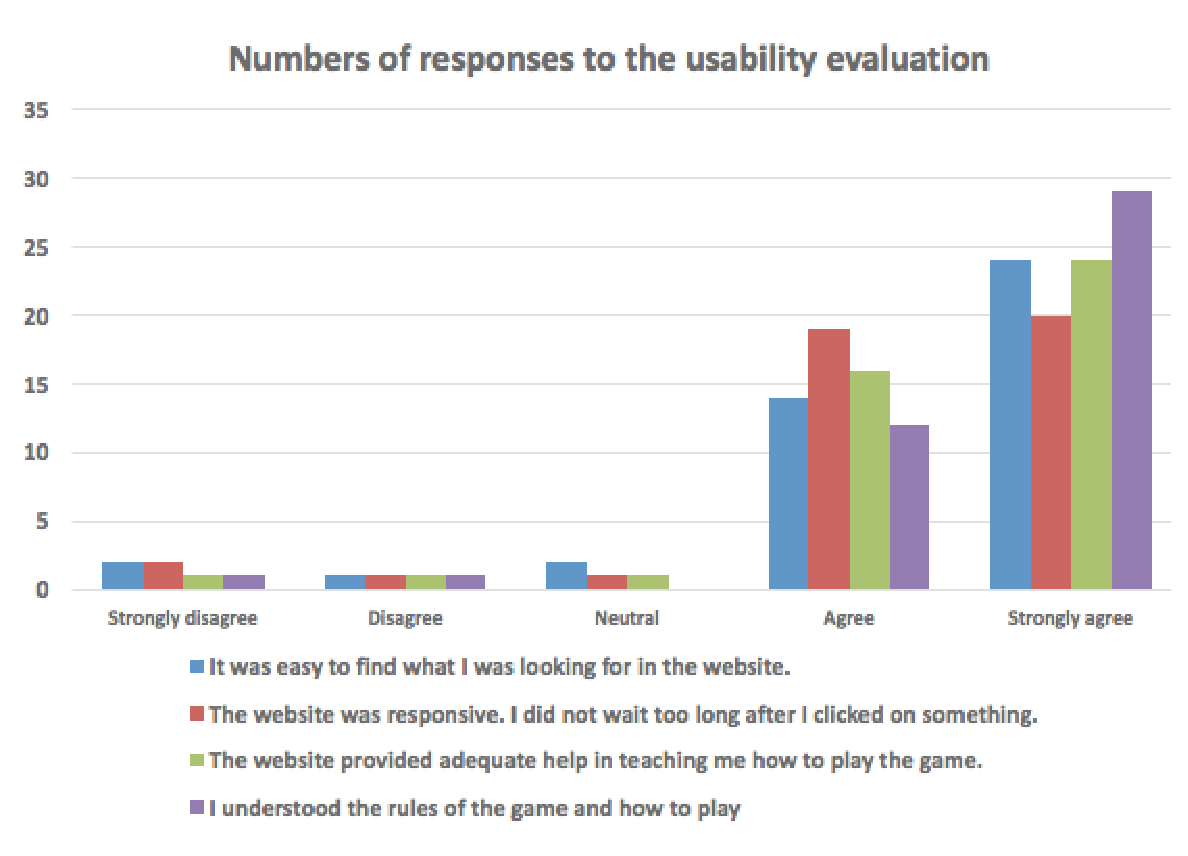
\includegraphics[height=2.2in, width=4.5in]{self-report-usability-2011.eps}}
		\subfigure[2014 Self-reported Usability Measurements(n=18)]{\label{fig:self-report-usability-2014}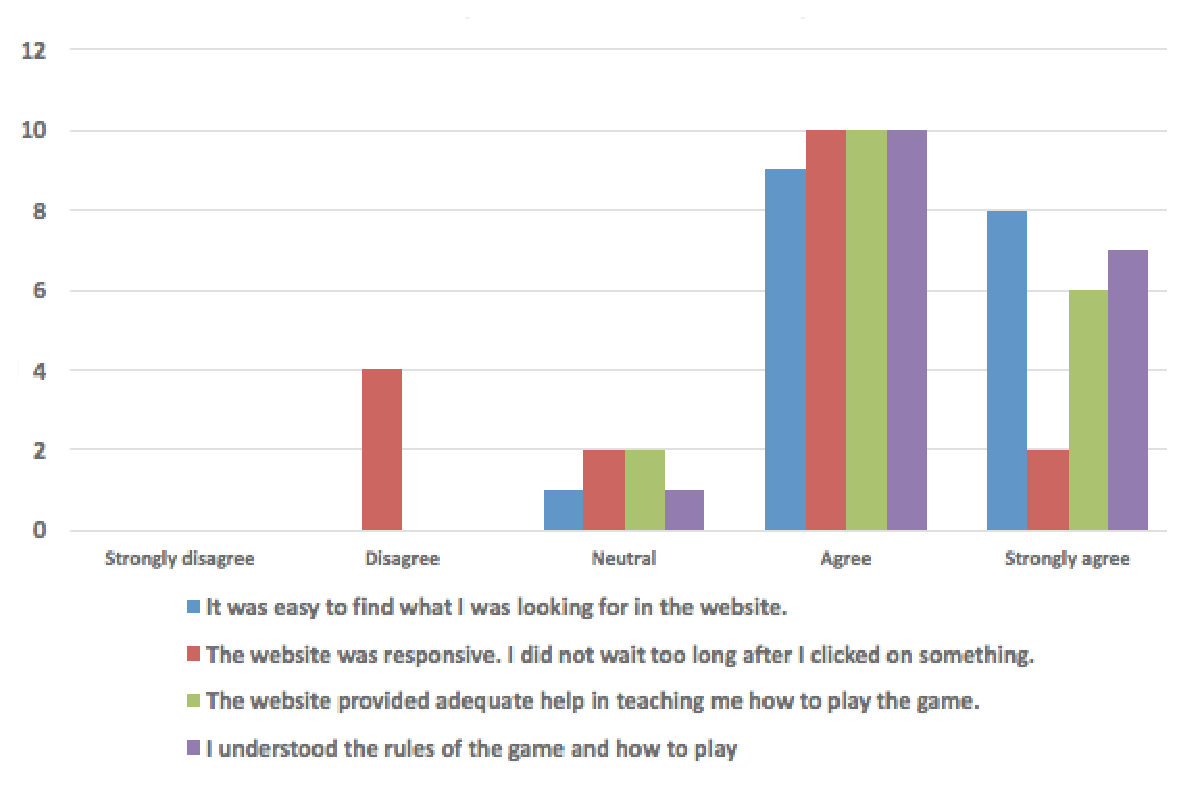
\includegraphics[height=2.4in, width=4.5in]{self-report-usability-2014.eps}}
		\caption{Self-reported Usability Measurements in 2011 KC and 2014 KC}
		\label{fig:self-report-usability-2011-2014}
\end{figure}

The majority of the players reported that they agreed the usability of the website is good with one exception of responsiveness from the 2014 responses. 4 out of 18 players (22\%) of the 2014 KC reported that they considered the website is not very responsive. Compared to the result of the 2011 KC, this indicates a perceived performance downgrade in the 2014 KC website.

Another question was asked in the 2014 UHM KC survey regarding the issues encountered when using the website. 3 out of 18 responses (17\%) reported that the loading of the website page was slow. This confirms the responsiveness issues discovered in the survey question described above. Another issue reported is confusion regarding the scoreboard's display on the website. 3 out of 18 responses (17\%) reported that scoreboard's display kept changing so it is not easy to see rankings. 2 responses reported that some of the videos were not displayed. It was later discovered that the links to those videos were outdated.

In summary, the self-reported usability survey is a good tool to get feedback from the players of Makahiki regarding the usability of the game. It reveals that most of the usability in Makahiki is good. It discovered a few usability issues in 2014 KC such as the slow performance of certain pages,  the confusion of scoreboard display, and the broken links to the educational video.

\subsubsection{Engagement metrics}
\label{sec:player-engagement-result}

Based on the engagement metrics proposed in SGSEAM (\ref{Engagement metrics}), we calculated a variety of engagement metrics to assess the player's engagement level in the 2011 and 2012 UHM Kukui Cup challenges created by the Makahiki framework. The metrics are calculated by analyzing the website logs and the game data collected by the application. The results are shown in \autoref{fig:makahiki-engagement}.
    
\begin{table}[ht!]
  \centering
  \begin{tabular}{|p{0.3\linewidth}|c|c|c|c|c|c|}
    \hline
    \tabhead{\multirow{2}{*}{Measurement}} & \multicolumn{3}{c|}{\tabhead{2011 KC}} & \multicolumn{3}{c|}{\tabhead{2012 KC}}\\
     \cline{2-7}
    \tabhead{} & \tabhead{MIN} & \tabhead{AVG} & \tabhead{MAX} &  \tabhead{MIN} & \tabhead{AVG} & \tabhead{MAX}\\

    \hline
    Participation rate & 13\% & 37\% & 74\% & 19\% & 34\% & 64\%\\
    \hline
    Number of players per day & 43 & 85 & 147 & 0 & 12 & 130 \\
    \hline
    Play time per day & 1 min & 27.7 mins & 8.5 hours & 0 & 6.2 mins & 8.8 hours\\
    \hline
    Submissions per day & 32 & 266 & 1110 & 0 & 30 & 953\\
    \hline
    Social interactions per day & 51 &  208 & 468 & 0 & 31 & 502\\
    \hline
    Website errors per day & 0 & 0.6 & 4 & 0 & 2 & 458\\
    \hline
  \end{tabular}
  \caption{Engagement Metrics for 2011 and 2012 UHM Kukui Cup}
  \label{fig:makahiki-engagement}
\end{table}

The participation rate is the percentage of players who played the game. The 2011 UHM KC had a 37\% average participation rate, while the 2012 KC had 34\%. According to the report from the successful Oberlin College Energy competition \cite{petersen-dorm-energy-reduction}, 46\% of residents looked at the competition website at least once (based on the IP addresses of the web server requests). Because the Oberlin system did not support user accounts, the IP address may not be a very accurate method to identify unique players. The actual participation rate might be lower than 46\%. Compared to the average 11\% participation rate of Western Washington University's Go for Green challenge \cite{Mauney-thesis} and the 0.4\% participation rate of University of Southern California's Ecolympics challenge \cite{Sintov2011}, both the 2011 and 2012 UHM KC challenges had good participation. 

Over the 3 week challenge in the 2011 KC, an average player spent about 27.7 minutes per day on the website, while in the 24 week challenge in the 2012 KC, an average player spent about 6.2 minutes per day. Both instances had one player spending over 8 hours (8.5 and 8.8 respectively) on one day, which is quite significant amount of time for a student to spend in this kind of serious game. The daily minimum time spent on the 2011 KC is 1 minute which indicates that for every day during the challenge, there was at least one player who played at least 1 minute. The daily minimum time spent on the 2012 KC is 0 minutes. This indicates that there was at least one day when no player used the website.

In order to investigate engagement in more detail, I looked at engagement measurement in a time series format. \autoref{fig:timeseries-metrics} shows the timed measurements graph during the 2011 and 2012 Kukui Cup.

\begin{figure}[ht!]
  \center
  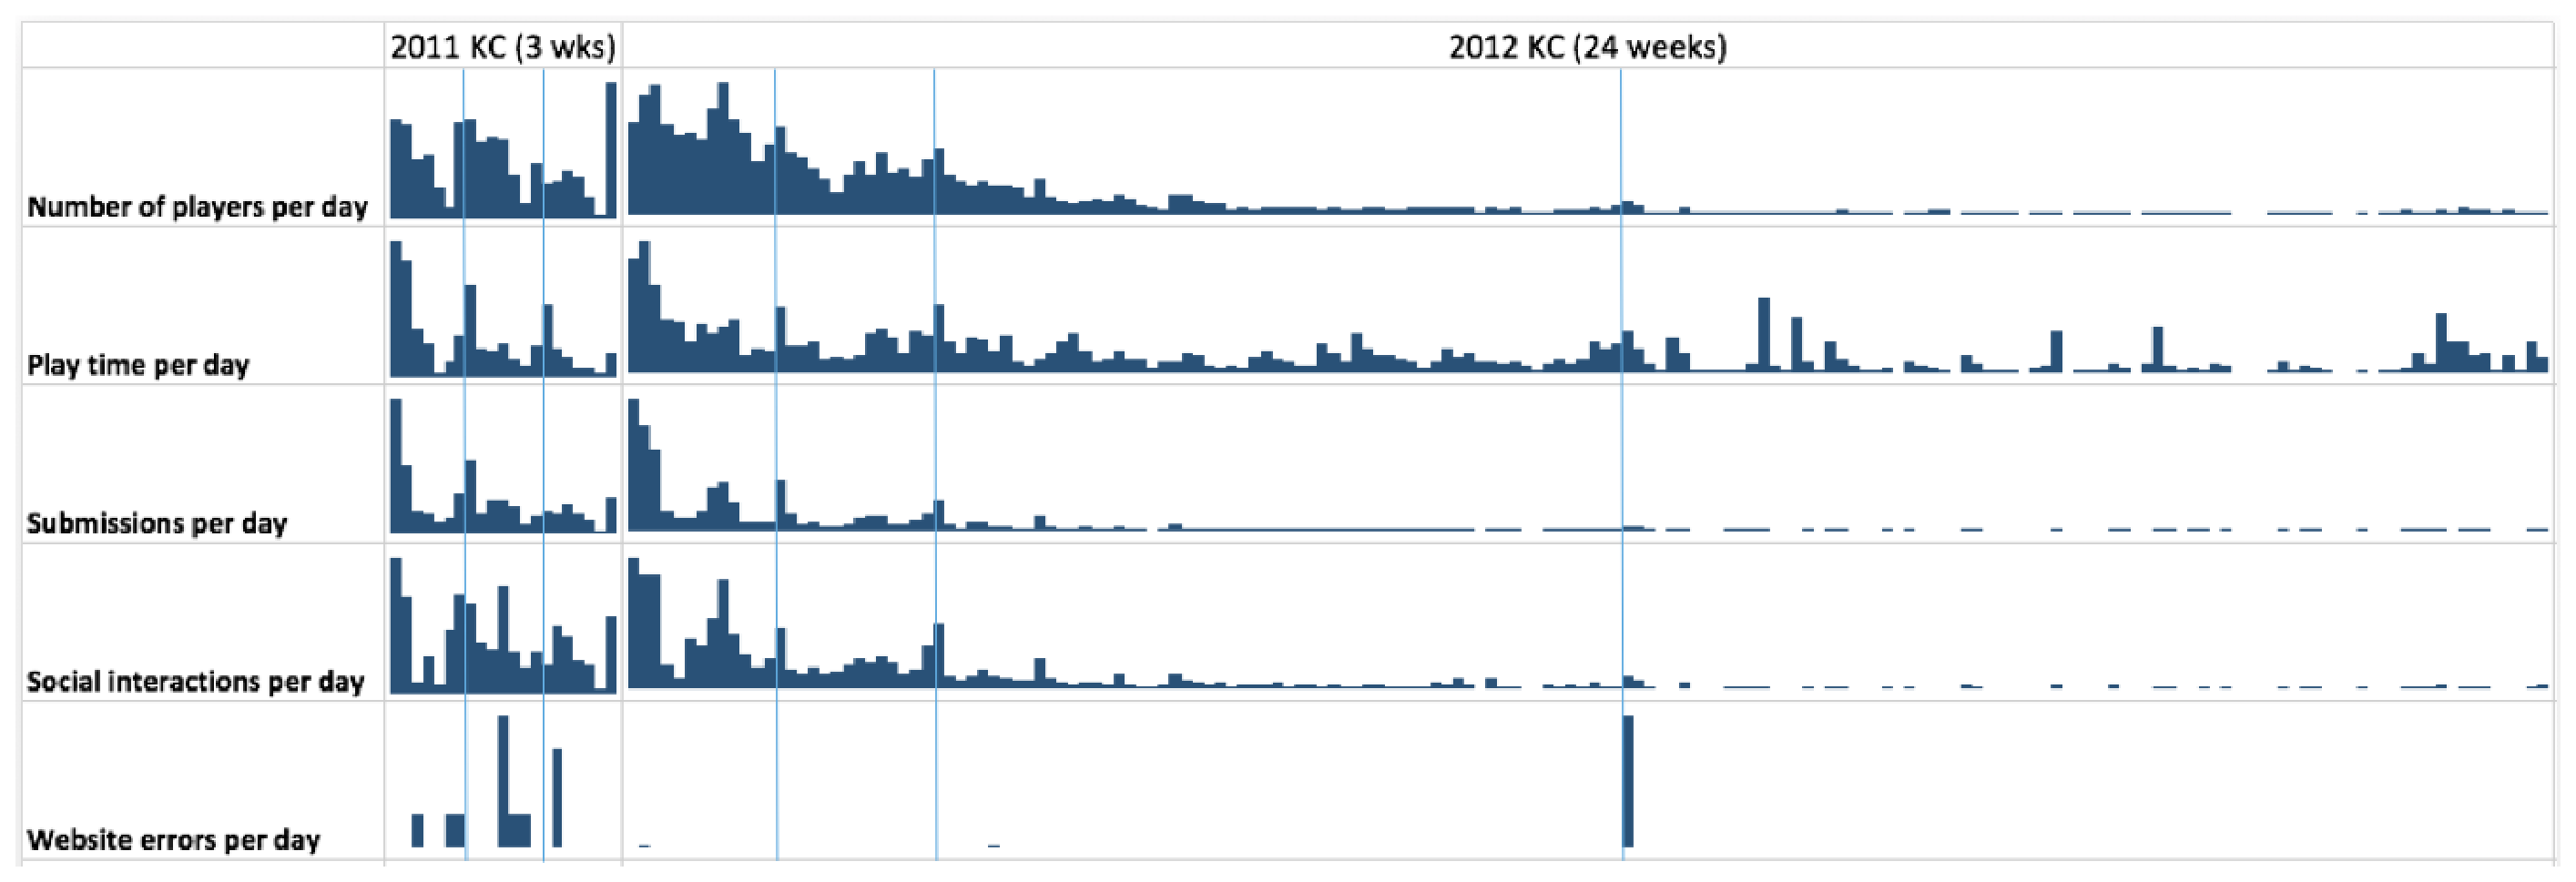
\includegraphics[height=2.6in,width=6in]{timeseries-metrics}
  \caption{Engagement Measurements during the 2011 and 2012 UHM Kukui Cup}
  \label{fig:timeseries-metrics}
\end{figure}

The vertical lines in the graphs indicates the division of the rounds for the 2011 and 2012 KC. In the 2011 KC, there are 3 rounds, each round lasting 1 week. In the 2012 KC, there were 4 rounds, the first and second round lasted 2 weeks each, and the third round lasted about 8 weeks, while the last round lasted about 12 weeks, for a total of 24 weeks for the 2012 KC. 

In addition to the daily number of players and daily play time which indicate the level of visits to the website or game, the daily submission and daily social interaction measurements indicate the level of deeper interactions with the game. We can see that during the 3 short weeks of the 2011 KC, the engagement patterns are similar in each week. The first few days have higher levels of interactions then decrease later into the week. There is a spike on the last day of the round, which may be due to last minute surge of interest in winning the round. 

We can also see that in the 2012 KC, the engagement level significantly dropped after the second round, which is 4 weeks after the beginning of the game. There are still some players spending time on the game but the number of submissions and social interactions had decreased significantly. The number of players decreased in the third round and decreased even more in the last round. It is interesting to see that there are still some amount of play time during the third and fourth round. A closer look at the data indicated that they are time spent from the few top players who have a chance to win the game. 

Although the website errors in the 2012 KC shown in \autoref{fig:makahiki-engagement} seems high, the detailed graph in \autoref{fig:timeseries-metrics} shows that the errors mostly happened during one day which is the day after the start of the last round. The investigation of the error in the log file revealed that they are due to a content configuration error in a newly available event in the last round. The error caused the players to not be able to submit the completion of the event to claim their points so they kept trying and encountered the error repeatedly. The error was corrected 2 hours later after the first such error occurred.

In summary, this analysis indicates that Makahiki was successful in achieving player engagement for a 3-to-4 week period in this kind of serious game. After this period, engagement seems to taper off. It is possible that engagement might stay high for a long period if there are a lot of activities throughout the period, but it requires substantial effort from game designers to create new activities and game managers to manage the game. More research must be done to understand how to maintain high levels of engagements over a long term period.

\subsection{Makahiki System Admin Assessment}
We used two approaches to assess the system administrators' experience with the Makahiki framework. They are the in-lab installation study and the post-hoc system admin interview.

\subsubsection{In-lab installation study}
\label{sec:sysadmin-in-lab-result}

In the in-lab installation study, the participants are the students in a serious game class (ICS691) in Spring 2013 in the information and computer sciences department at the University of Hawaii at Manoa. The students were tasked with installing the Makahiki system into their local computers as well as deploying to the Heroku cloud environment. A Google Form (described in \autoref{app:googleform-sysadmin}) was used to ask the students to record the time they spent completing each step and the problems they encountered. The students also provided feedback about their installation experiences in the form of blog posts. There were a total of 8 students who voluntarily participated in the experiments.  The participants were either senior undergraduates or graduate students majoring in Computer Science. 

In the local installation study, the results from the Google Form responses show that the average total time to successfully install Makahiki in their local computers was 1.4 hours, with a maximum time of 2 hours and a minimum time of 0.9 hour. \autoref{table:local-install-time} and \autoref{fig:local-install-time} shows the average time and their percentage distributions of each step in the local installation study.

\begin{table}[ht!]
  \centering
  \begin{tabular}{|p{0.3\linewidth}|P{0.45\linewidth}|P{0.14\linewidth}|}
    \hline
    \tabhead{Category} & \tabhead{Installation Tasks} & \tabhead{Average Time (minutes)} \\
    \hline
    Setup runtime environment & Install Python, C compiler, Git, Pip and Virtual environment & 10.0 \\
    \hline
    Install dependencies & Install Python Imaging Library, Memcache, required python packages & 29.4 \\
    \hline
    Install and configure database & Install and configure PostgreSQL & 37.5 \\
    \hline
    Download the software & git clone from Github & 7.5 \\
    \hline
    Install the software & setup environment variables, run initialize\_instance script & 26.8 \\
    \hline
    Start the server and verify & start the server and verify the server running correctly & 2.5 \\
   \hline
    \end{tabular}
  \caption{Average time (minutes) for local installation steps (n=8)}
  \label{table:local-install-time}
\end{table}
    
\begin{figure}[ht!]
  \center
  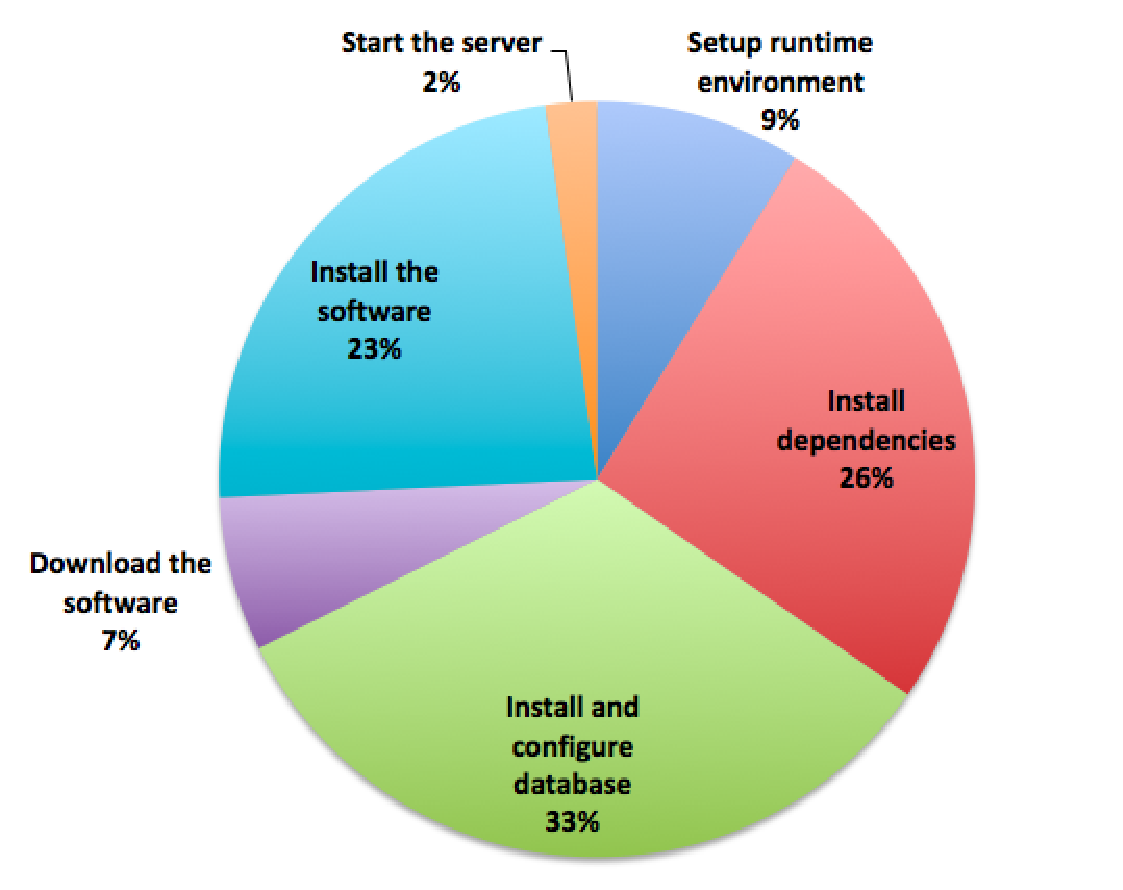
\includegraphics[width=0.6\columnwidth]{install-time}
  \caption{Average time for local installation steps (n=8)}
  \label{fig:local-install-time}
\end{figure}

The descriptive problems reported by the students in both the Google Form
and their blog posts were coded and categorized. The analysis results are shown in \autoref{fig:local-makahiki-install}.

\begin{table}[ht!]
  \centering
  \begin{tabular}{|p{0.7\columnwidth}|c|}
    \hline
    \tabhead{Problem encountered} & \tabhead{Number of participants} \\
    \hline
    Cannot find configuration file to edit during database installation  & 4 \\
    \hline
    Documentation of install script is confusing about creation of the DB user & 2 \\
    \hline
    More parts of installation could be covered by install script & 2 \\
    \hline
  \end{tabular}
  \caption{Makahiki local installation issues reported (n=8)}
  \label{fig:local-makahiki-install}
\end{table}

From the above analysis, we identified that the ``Install and configure database'' step of the local installation has the longest average time. It also has the most problems reported from the participants. This assessment determines the areas for future improvement for the local installation are (1) to improve documentation on DB installation, and (2) to improve the install script to automate more installation tasks.

In the Heroku cloud installation study, the results from the Google Form responses revealed different experiences. The average total time to successfully install Makahiki in the Heroku cloud environment was 1.9 hours, with a maximum time of 3.6 hours and the minimum time of 0.7 hour. \autoref{table:heroku-install-time} and \autoref{fig:heroku-install-time} shows the average time and their percentage distributions of each step in the Heroku cloud installation study.

\begin{table}[ht!]
  \centering
  \begin{tabular}{|P{0.28\linewidth}|P{0.48\linewidth}|P{0.14\linewidth}|}
    \hline
    \tabhead{Category} & \tabhead{Installation Tasks} & \tabhead{Average Time (minutes)} \\
    \hline
    Setup cloud environment & Install Heroku client, add ssh keys to Heroku, verify Heroku account, setup Amazon S3 & 50.6 \\
    \hline
    Download software & git clone from Github & 6.3 \\
    \hline
    Deploy to cloud & setup environment variables, run initialize\_instance script & 39.5 \\
    \hline
    Start the server and verify & start the server and verify server running correctly & 29.4 \\
        \hline
  \end{tabular}
  \caption{Average time (minutes) for Cloud installation steps (n=8)}
  \label{table:heroku-install-time}
\end{table}
    
\begin{figure}[ht!]
  \center
  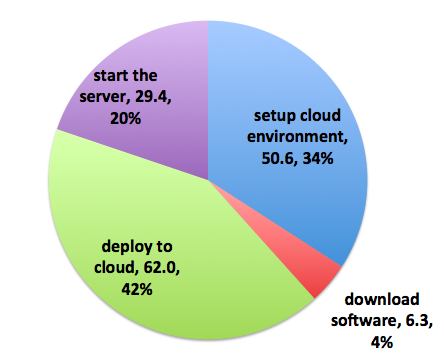
\includegraphics[width=0.6\columnwidth]{install-time-cloud}
  \caption{Average time for cloud installation steps (n=8)}
  \label{fig:heroku-install-time}
\end{figure}

\autoref{fig:heroku-makahiki-install} shows the result of the analysis from
the blog post feedbacks regarding participants' cloud installation experiences.

\begin{table}[ht!]
  \centering
  \begin{tabular}{|p{0.7\columnwidth}|c|}
    \hline
    \tabhead{Problem encountered} & \tabhead{Number of participants} \\
    \hline
    confusion in setting up Amazon S3 & 5 \\
    \hline
    took a long time to upload application to Heroku & 3 \\
    \hline
    needing to use the virtual environment is not documented & 3 \\
    \hline
    Failure messages are buried in the verbose script output thus overlooked & 2 \\
    \hline
  \end{tabular}
  \caption{Makahiki cloud installation issues reported from blog posts (n=8)}
  \label{fig:heroku-makahiki-install}
\end{table}

From the above analysis, we identified that the ``Setup cloud environment'' step has the
longest average time. It also has the most participant-reported problems regarding confusion in setting up Amazon S3. This assessment reveals the areas for future improvement for the cloud installation are: (1) to improve documentation on cloud environment setup; (2) to improve usability of the install script; and (3) develop tools to verify and diagnose the environment setup.

In summary, the in-lab installation study identified database installation, documentation and the usability of the install script as the weak points in the process of installing Makahiki.  Otherwise, SGSEAM indicates generally positive results regarding Makahiki installation.

\subsubsection{Post-hoc System Admin Interview}
\label{sec:sysadmin-interview-result}

In order to gain insight into the experience of real world system admins who use Makahiki, I performed interviews with the system admin of the Hawaii Pacific University (HPU) Kukui Cup challenges and analyzed the problems they encountered during software installation and system administration. The HPU KC server software was installed by the system administrator from the HPU IT department with assistance from the Makahiki development team. The installation was performed in the HPU local IT infrastructure and included integration with the HPU LDAP server and their email server.  During the installation, issues encountered were communicated through emails and phone calls between the administrator and Makahiki development team. The interview took place after the challenge. 

The data about the system admin experience was compiled and listed in \autoref{fig:makahiki-install-hpu2012} and \autoref{fig:makahiki-install-hpu2013} for the 2012 and 2013 HPU KC instances respectively. The working days to complete is the working days for the HPU system admin to complete an  installation task. During those working days, the system admin might have other work responsibilities not related to the Makahiki software installation. The actual time spent working on the Makahiki installation might be less than the reported working days, but this data may reflect the actual work load in a typical IT organization, so it is still an indication of relative time spent on the different installation tasks.

\begin{table}[ht!]
  \centering
  \begin{tabular}{|P{0.28\columnwidth}|P{0.1\columnwidth}|p{0.5\columnwidth}|}
    \hline
     \tabhead{Installation Task} &
     \tabhead{Time to Complete} &
     \tabhead{Issues and Problem Encountered} \\
    \hline
     Install and startup server & 5 days & error in installing the runtime environment virtualenvwrapper\\
    \hline
    Install image library & 1 day & error in displaying JPG image during testing \\
    \hline
     Integrate with HPU LDAP server &  20 days &  need to install ldap libraries; need to create a special bind user to connect to the ldap server; use the correct ldap DN; HPU ldap server use non-standard way to identify user so the Makahiki software need to update to support HPU's server settings \\
    \hline
    Integrate with HPU Email Server & 2 days & need to create a special email account for KC admin;  HPU email server reported error due to the "from" parameter is not the same as the email account so the Makahiki software need to fix to support HPU's email. \\
    \hline
    Update the Makahiki software & 1 day & none \\
    \hline
    Use SSL & not complete & need to procure the SSL certificate; the SSL certificate acquired by HPU does not have a trusted CA, it is decided that the competition will start without SSL \\
    \hline
    Total & 29 days & \\
    \hline
  \end{tabular}
  \caption{Installation Issues in HPU 2012 KC }
  \label{fig:makahiki-install-hpu2012}
\end{table}

\begin{table}[ht!]
  \centering
  \begin{tabular}{|P{0.28\columnwidth}|P{0.1\columnwidth}|p{0.5\columnwidth}|}
    \hline
     \tabhead{Installation Task} &
     \tabhead{Time to Complete} &
     \tabhead{Problem Encountered} \\
    \hline
     Startup from last year's Vmware image & 1 day &  none\\
    \hline
     Makahiki software upgrade & 1 day & need to recreated database migration script due to HPU still use older Postgresql DB version. \\
    \hline
    Integrate with HPU LDAP server & 1 day  & not able to login because the HPU LDAP server changed to use a new directory structure \\
    \hline
     Integrate with the new LDAP server &  1 day &  need to reconfigure to use the new LDAP server\\
    \hline
    Use HPU Email Server & 2 days & not able to send email because the HPU email server configuration change. \\
    \hline
    Total & 6 days & \\
    \hline \end{tabular}
  \caption{Installation Issues in HPU 2013 KC }
  \label{fig:makahiki-install-hpu2013}
\end{table}

The data shows that the the configuration to use HPU's LDAP server and email server are the most difficult tasks. It took a comparable large amount of time to install the LDAP libraries, create the ldap account, test the correct configuration and eventually discover that the Makahiki software needed to be modified to support HPU's special server settings. 

Once the integration with the HPU's local infrastructure was completed in 2012, the 2013 experience was much easier, and the LDAP and email server configuration changes were completed quickly. 

When asked about the experience of maintaining the Makahiki server, such as backup and monitoring, the system admin answered that it was fairly straightforward to perform the backup. Since the server was built on the VMWare virtual machine, he used the snapshot function in the VMware management console to perform the daily backup. The backed up image was successfully used in 2013 as the starting point for the 2013 KC instance without the need to re-install the software. The system admin did not do any monitoring and relied on the game designer and manager to report any issues to him. During the running period of the two challenges, there was no report of performance issues. Only one issue related to system installation was reported by the game designer during the testing of the 2012 HPU KC. It is the JPG image support library not being installed. It took 1 day for the sys admin to correct the problem.

In summary, the SGSEAM post-hoc system admin interview approach revealed difficulty in integrating Makahiki with an organization's LDAP and email server as well as using SSL in a local installation scenario. As a result, it is advisable to plan well ahead and allow ample time (at least one month) for these tasks.  Compared to the in-lab installation study, the database installation is not an issue for the real world system admin. It is probably due to the IT system admin skill and experience difference between  IT professionals and graduate students. 

\subsection{Makahiki Game Designer Assessment}

\subsubsection{In-lab game design study}
\label{sec:designer-in-lab-result}

The in-lab game design study was also performed using the UHM ICS691 course in Spring 2013. One of the class assignments for the students in the experiment was to design a serious game using the Makahiki framework. We asked the students to follow specific design steps and record the time required and any problems encountered during their design process, using a Google Form outlined in \autoref{app:googleform-design}. In addition, students were asked to provide feedbacks about their
design experiences in the form of blog posts. 

The game designer assessment was generalized into 7 tasks corresponding to
distinct types of administrative tasks and game design planning. The time for each task is
calculated from the Google Form responses. 

There were a total of 8 students who voluntarily participated in the experiments. The most time consuming task was ``Smart Grid Game Design", which took an average of 107.9 minutes (56\% of total time) to complete, while the least time consuming tasks was ``Raffle Game Design", which took an average of 7.9 minutes (7\% of total time) to complete. \autoref{table:design-time} and \autoref{fig:design-time} shows the average time and their percentage distributions for each design tasks.

\begin{table}[ht!]
  \centering
  \begin{tabular}{|P{0.3\linewidth}|P{0.45\linewidth}|P{0.14\linewidth}|}
    \hline
    \tabhead{Category} & \tabhead{Design Tasks} & \tabhead{Average Time (minutes)} \\
    \hline
    Configure challenge settings & customize challenge name, logo; define teams, setup users, select games & 46.5 \\
    \hline
    Design the resource goal game & customize the default energy goal game with manual data input & 5 \\
    \hline
    Design the smart grid game & add a new level to the existing smart grid game with multiple types of actions and unlocking sequence & 107.9 \\
    \hline
    Design the top score game & add new prizes to the existing top score game & 10.7 \\
    \hline
    Design the raffle game & add new raffles to the existing raffle game & 7.9 \\
    \hline
    Design the badge game mechanic & add new badges with awarding condition & 13.6 \\
   \hline
    \end{tabular}
  \caption{Average time (minutes) for design tasks (n=8)}
  \label{table:design-time}
\end{table}
    
\begin{figure}[ht!]
  \center
  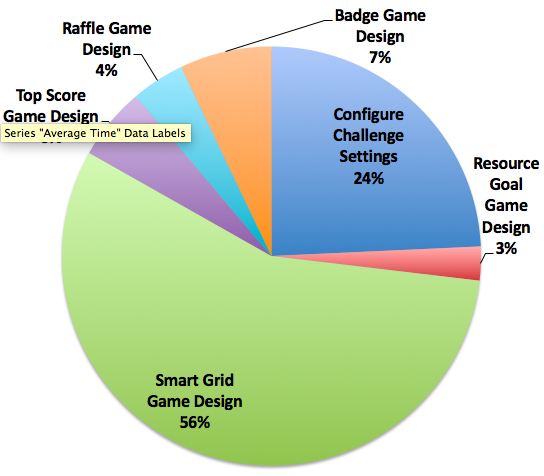
\includegraphics[width=0.6\columnwidth]{design-time}
  \caption{Average time for design tasks (n=8)}
  \label{fig:design-time}
\end{figure}

Problems reported in the blog post feedbacks were analyzed. The results are shown in \autoref{fig:makahiki-game-design}.

\begin{table}[ht!]
  \centering
  \begin{tabular}{|p{0.7\columnwidth}|c|}
    \hline
    \tabhead{Problem encountered} &
    \tabhead{Number of participants} \\
    \hline
    Difficulty in understanding predicate system and unlock condition & 7 \\
    \hline
    A bug that prevented users with usernames containing capital letters from logging in & 2 \\
    \hline
    A bug in the processing of Ajax queries & 1 \\
    \hline
    Difficulty in generating event attendance codes for game activities & 1 \\
    \hline
  \end{tabular}
  \caption{Makahiki Game Design Analysis, (n=8)}
  \label{fig:makahiki-game-design}
\end{table}

In summary, the SGSEAM in-lab game design study revealed the two most time consuming tasks in  Makahiki design are ``Smart Grid Game Design'' and ``Configure Challenge Settings''. Issues encountered in ``Smart Grid Game Design'' include: 1) difficulty and lack of documentation on the predicate system used to define dependencies between game activities, and 2) difficulty in generating event attendance codes for game activities. Issues encountered in ``Configure Challenge Settings'' include: 1) a bug in the processing of Ajax queries caused by consecutive clicks on the same interface button, and 2) a bug that prevented users with usernames containing capital letters from logging in.

\subsubsection{Post-hoc Game Designer Interview}
\label{sec:designer-interview-result} 

In order to gain insight into the experience of a real world game designer who uses the Makahiki software to design a serious game, I performed interviews with the game designers of the two Kukui Cup challenges in Hawaii Pacific University (HPU) and East-West Center (EWC) in the year of 2012. The game designer for HPU is the sustainability coordinator for the Hawaii Pacific University; while the game designers for EWC are two sustainability coordinator for the East-West Center Participant Association. We asked them about their game designing experiences using the Makahiki game design interface. In addition to the interview data, Makahiki system log file and email exchanges were analyzed to identify the problems encountered during the game design process.

\autoref{fig:hpu-design} and \autoref{fig:ewc-design} lists the game design experience with Makahiki for the 2012 HPU and 2012 EWC Kukui Cup instances respectively. 

\begin{table}[ht!]
  \centering
  \begin{tabular}{|P{0.5\columnwidth}|P{0.4\columnwidth}|}
    \hline
    \centering \tabhead{Problem encountered} &  \tabhead{Cause} \\
    \hline
    Error displaying the prize page after adding a prize  & Makahiki software did not validate the prize parameter inputted \\
    \hline
    The introduction video referenced to previous year &  The introduction video should be made generic so it could be reused over years \\
    \hline
    Error when users saved their profile in the profile page & Python Image Library was not installed correctly\\
    \hline
    Confusion of the event code generation & The admin interface to generate the event code was not intuitive\\
    \hline
    Don't know how to creating external link in Kukui Cup Activities description & The markup language for activity description is not WYSIWYG \\
    \hline
    Smartgrid layout did not change immediately after the settings changed & The cache was not clear automatically when setting changed\\
    \hline
  \end{tabular}
  \caption{Makahiki Game Design Experiences in 2012 HPU Kukui Cup}
  \label{fig:hpu-design}
\end{table}

\begin{table}[ht!]
  \centering
  \begin{tabular}{|P{0.5\columnwidth}|P{0.4\columnwidth}|}
    \hline
    \centering \tabhead{Problem encountered} & \tabhead{Cause} \\
    \hline
    Confused when generating the confirmation code  & the admin interface was not intuitive \\
    \hline
    Don't know how to use video other than youtube &  Makahiki software only supported youtube video id \\
    \hline
    Forgot to change the default commitment period & the default was meant for testing and not typical\\
    \hline
    Not able to delete the FAQ widget from help page & the admin interface to find the name of the widget on a page is not intuitive \\
    \hline
  \end{tabular}
  \caption{Makahiki Game Design Experiences in 2012 EWC Kukui Cup}
  \label{fig:ewc-design}
\end{table}

One EWC designer responded that ``It is easy to create the smartgrid game, putting (up) the video etc. The interface was easy to use''. She also mentioned that it is ``Just a little bit time consuming''.

In summary, the general responses from the game designers of the real world Makahiki instances are positive. There was some confusion in the usability of the game design admin interface, especially in the area of generating the event confirmation code and the user interface is not intuitive enough for easy game content creation. Both the in-lab study and post-hoc interviews revealed the confusion in the event confirmation code generation interface.

\subsection{Makahiki Game Manager Assessment}
\label{sec:manager-interview-result} 

In order to gain insight into the experience of real world game managers who use the Makahiki software to manage a serious game, I performed interviews with the game managers of the two Kukui Cup challenges at Hawaii Pacific University (HPU) and East West Center (EWC) in the year 2012. The game manager for HPU is the sustainability coordinator for the Hawaii Pacific University; while the game managers for EWC are two sustainability coordinators for the East-West Center Participant Association. They are also the game designers for their Kukui Cup instances. We asked them about their game management experiences using the Makahiki admin
interface. The Makahiki instance log files and email exchanges between the game managers and us were also analyzed in order to identify the problems encountered during game management process.

\autoref{fig:hpu-ewc-manage} shows the reported problems encountered during the game management in the 2012 HPU and  EWC Kukui Cup instances. 

\begin{table}[ht!]
  \centering
  \begin{tabular}{|P{0.4\columnwidth}|P{0.4\columnwidth}|P{0.1\columnwidth}|}
    \hline
    \centering \tabhead{Problem encountered} &
    \centering \tabhead{Cause} & 
    \tabhead{Reporting Instance} \\
    \hline
    Not easy to find the event confirmation code  & the admin interface to view the event confirmation code was not intuitive & HPU and EWC \\
    \hline
    Error when clicking on the "save and add another" button in the approval admin interface &  the approval admin interface should remove the "save and add another" button & HPU and EWC \\
    \hline
    Some status data disappeared after the competition ended & Makahiki software bug & HPU\\
    \hline
    Missing two days worth of energy and water data & did not enter the manual energy and water data in time & EWC\\
    \hline
    Intermittently unable to access the website  & there was a DNS problem with the domain name registrar & EWC\\
    \hline
    Did not support sending out email daily about the current status of the game & software not support yet & EWC \\
    \hline
    Need to make the game site available to player after the competition over & software not support yet & EWC \\
    \hline
  \end{tabular}
  \caption{Makahiki Game Managing Experiences in 2012 HPU and EWC Kukui Cup}
  \label{fig:hpu-ewc-manage}
\end{table}

When asked if it was easy to approve the player's submissions, the HPU game manager responded that it was ``very easy''. EWC game managers responded that ``the interface was easy''.

Regarding the approval process, HPU game manager responded that he did not encounter any problems and there was no need to spend a lot of time. He made sure that player submissions were either approved or rejected within 12 hours. He also discovered a useful ``approve in batch'' feature in the approval interface without help from the Makahiki support team.  Both HPU and EWC game managers found that the ``Status'' game analytics page was very helpful. It was their main tool to monitor and get a sense of the status of the game.

We discussed some special issues of the game managing process in the EWC instance. The EWC instance did not use smart meters so the resource usage data had to be inputted manually by the game manager. They reported that it was a hassle to manually enter the data. The access to the water meter device was especially not pleasant.  A second issue with the EWC instance was that, because the number of players in the two competing teams were significantly different, a simple aggregation of one team's player total points did not make sense for the team points. The energy and water consumption were also largely affected by the number of residents in the building represented by the team. A few days after the game started, the game manager realized the issues need to be addressed otherwise the competition would not be fair. We modified the Makahiki software to support the per-capita in team point calculation and update the EWC instance before the first round of the game ended. A third issue with the EWC instance was the process of player registration. Typically, player accounts in Makahiki are created by game managers before the game and do not normally change during the game. In the case of EWC instance, the team rosters were not available to the game manager so they had to use a google form to sign up players. In many cases, new players were signed up during several events during the game. The game managers had to created accounts for the new players manually in the middle of the game.

In summary, SGSEAM uncovered a few problems with Makahiki game management using the interview
approach. We realized that the confidence level of this assessment approach is low because of the availability of only a few data points. An experimental study approach or performing interviews with 
more game managers would increase the confidence level of the assessment. Nevertheless, the interview approach provided useful insights into the real-world game management experience in this kind of serious game context.

\subsection{Makahiki Developer Assessment}
\label{sec:developer-in-lab-result} 

We assessed the developer experience using an in-lab game development study. The UHM serious game development course, ICS691 in Spring 2013, was used for the experiment. The participating students were asked to complete the assignment to develop an enhancement to Makahiki.  This involved setting up a development environment, following a tutorial to create a ``Hello World'' widget using Makahiki, and finally, developing an enhancement to extend the functionality of Makahiki which required five  development tasks.  The students were asked to submit their development source code to the public source code repository (GitHub) and write a blog post to discuss their efforts and experiences in completing development activities. The estimated completion time was 10 to 30 hours. The students were told to complete as much as possible and if they could not complete all the activities, they should report in their blog posts what they could not complete. The blog posting should also discuss the parts of the enhancement exercise that they found easy to complete, the parts they found hard to complete, and their recommendations for how the Makahiki framework could be improved to support such enhancement activities more easily in the future. 

The \autoref{table:makahiki-dev} shows the results of the in-lab game development study after analyzing the blog posts and the source codes submitted by the participants. 

\begin{table}[ht!]
  \centering
  \begin{tabular}{|p{0.5\columnwidth}|c|c|}
    \hline
    \tabhead{Development Task} &
    \tabhead{Number of completion} & 
    \tabhead{Reported Difficulty}\\
    \hline
    Setup development env & 8 & easy\\
    \hline
    Create the ``Hello World'' widget & 8 & easy\\
    \hline
    Update score\_mgr class to support groups. & 7 & easy \\
    \hline
    Create a group scoreboard widget. & 7 & hard \\
    \hline
    Create a group resource widget. & 4 & hard\\ 
     \hline
    Create a group prize widget. & 2 & hard\\
     \hline
    Create two group statistics widgets for the status page & 1 & hard\\
    \hline
  \end{tabular}
  \caption{Makahiki Game Development Experience, (n=8)}
  \label{table:makahiki-dev}
\end{table}

All 8 students reported that the first three tasks of setting up the environment, creating the  ``Hello world'' widget and extending the score\_mgr class was easy, while the rest of the enhancements were hard. Only one student was able to successfully complete all the required enhancement developments, while most of them were able to successfully complete the reported easy tasks. 

\autoref{table:makahiki-dev-problems} shows the reported problems encountered during game development. The main problem students reported was the lack of documentation for the development libraries.  All students reported that they spent at least 10 hours working on the assignment. 5 students stated that they had spent more than the assignment estimated hours and had to move on without completing the assignment. 

\begin{table}[ht!]
  \centering
  \begin{tabular}{|P{0.8\columnwidth}|P{0.14\columnwidth}|}
    \hline
    \tabhead{Problem encountered} &
    \tabhead{Number of participants}\\
    \hline
     Lacking and confusing documentation, not consistent, the screenshot does not match & 8 \\
    \hline
    Spent more than the assignment estimated hours & 5 \\
    \hline
    Don't know how to add the widgets to the Heroku instance & 2  \\
    \hline
    Help topic is hard to change & 1 \\
    \hline
    Confusion between INSTALLED\_APPS and INSTALLED\_WIDGET\_APPS & 1\\ 
     \hline
    Lots of files in the original Prizes folder, not sure what was needed and what was not & 1 \\
     \hline
    Had trouble getting the templates to redirect to the right place & 1\\
    \hline
    Have to find out how to ``subclassing'' a widget by looking at the source code & 1 \\
    \hline
    Had to use stackoverflow to get answer for env and Django issues & 1 \\
    \hline
    Learning the code base, a lot to digest, e.g. Django, template, aggregation & 1 \\
    \hline
  \end{tabular}
  \caption{Makahiki Game Development Problems, (n=8)}
  \label{table:makahiki-dev-problems}
\end{table}

The following are the list of comments and suggestions for ways to enhance the Makahiki support to developing enhancements to the framework:

\begin{figure}[ht!]
\begin{mybox}
\begin{compactenum}
	\item ``better documentation, add type hierarchy diagram''
	\item ``wished for a bit more of a high-level overview of how widgets should work''
	\item ``how to develop with the heroku instance is not document; this guide could use more specifics, and updating to adhere to changes in the program.''
	\item ``Sometimes a method returned a dictionary, but the documentation did not give the dictionary keys''
	\item ``have a database model diagram''
\end{compactenum}
\end{mybox}
\caption{Suggestion for Makahiki Game Development support}
\label{fig:develop-suggestion}  
\end{figure}

One student stated in his blog that he decided to choose the Makahiki
framework to develop his own serious game because of Makahiki's features and the possibility
of reducing development effort by using the framework. 

In summary, the SGSEAM in-lab game development study revealed significant problems with developer efficiency in Makahiki. The problems reported in this assessment are very helpful to address the areas of improvement regarding Makahiki's support for developing game enhancements.

\subsection{Assessment Report}

After the above assessments were performed for each SGSEAM stakeholder in Makahiki, an assessment report was created as the final deliverable of the SGSEAM assessment of Makahiki. This report is included in \autoref{app:makahiki-improvement-report}. It  describes the strengths of the Makahiki framework that need to be maintained, the weakness areas that can be improved, and the recommended actionable steps on how to improve from each stakeholder's perspective. 

\subsection{Summary}

This section described the application of SGSEAM to assess the strengths and weaknesses of the Makahiki framework. The {\em in-vivo} approaches were applied to the real-world Kukui Cup challenges created by the Makahiki framework, while the {\em in-vitro} approaches were applied to the UHM ICS691 serious game course to assess Makahiki from the perspectives of the five serious game stakeholders identified by SGSEAM: players, system admins, game designers, game managers and game developers.

The SGSEAM assessment results were described in the format of an assessment report (\autoref{app:makahiki-improvement-report}) which lists the strengths and weaknesses of Makahiki, and the recommended improvement actions. The report itemizes the areas of the Makahiki framework that need improvement from the five stakeholders' perspectives. SGSEAM revealed that the major strengths of Makahiki are the ability to create an engaging and effective serious game for an organization, and the ability to provide an easy-to-use interface for game designers and managers. SGSEAM revealed the major weaknesses of Makahiki are difficulty in developing new enhancements to extend the framework from a game developer's perspective, difficulty to integrate external services such as LDAP and email server from a system admin's perspective, and the lack of WYSIWYG content authoring tool from a game designer's perspective.

\section{Discussion}

This chapter described the results of Makahiki being used to create and manage 7 real-world sustainability games by 4 organizations. These games were created in various configurations and hosting environments. The successful creation of these serious game instances provides evidence that Makahiki can be successfully tailored to the needs of these organizations. The Makahiki framework performed well in the context of university settings, approximately 1000 player population and support a certain type of smart meters, and authentication. It is unknown whether the framework is able to scale to a vastly different population such as residential, or more than 1000 players. We are actively looking for opportunities to expand Makahiki to different population and settings, to understand the design capability of Makahiki.

Most of the Makahiki experiences were in the context of university settings with university residence hall and college students. Although we had a small pilot instance targeted at an elementary school, the experience was limited, partly due to the piloting and the effort to carry out the assessment with human subjects involving minors. The expanding of player population beyond college students may have impacts on the effectiveness and usability of the framework besides the education content. For example, elementary students may find the game interface confusing with the complicated unlock mechanism in the SmartGrid game. Expanding Makahiki into other geographical locations may require software modifications to support internationalization both in the interface and content support. 

This chapter also described the application of SGSEAM to assess the strengths and weaknesses of the Makahiki framework. The {\em in-vivo} approaches were applied to the real-world Kukui Cup challenges created by the Makahiki framework, while the {\em in-vitro} approaches were applied to the UHM ICS691 serious game course to assess Makahiki from the perspectives of the five serious game stakeholders identified by SGSEAM: players, system admins, game designers, game managers and game developers. The assessment identified the strengths and weaknesses of Makahiki as a serious game framework for sustainability, and produced an improvement action report with recommendations on how to improve the framework with respects to the different serious game stakeholder's perspectives. 

The application of SGSEAM to Makahiki effectively identified the strengths and weaknesses of Makahiki and provided improvement suggestions to Makahiki developers. It also revealed the strengths and weaknesses of SGSEAM as an assessment method. 

One weakness of SGSEAM is that the process can be expensive and time consuming. Although the approach does not mandate you to perform all the assessment approaches proposed in SGSEAM, it is desirable to perform as many approaches as possible, depending on the resources available. In the case of applying SGSEAM to Makahiki, it required a large amount of effort to carry out different assessment approaches for each stakeholder. The data collection and data analysis were also time consuming. The fact that we were not able to convince Lucid design group to do the SGSEAM assessment could be an indication that the cost of SGSEAM process is also high from Lucid's view.

While the comprehensive SGSEAM assessment are expensive, the design of SGSEAM does allow the flexibility of picking any one of the approaches or any one of the stakeholders, in the case of only some of the stakeholders' experiences are the main concerns from the framework developers. Because of the SGSEAM approaches are additive, the more approaches are assessed, the more confidence the assessment could be. This flexibility of choosing from a set of additive approach is a strength of the SGSEAM.

The categorization of the five serious game stakeholders is a strength of SGSEAM. It forces the assessors or the developers of a serious game framework to think in term of these categories when looking for improvements for their framework. The 3-step process of SGSEAM should also help the assessors to carry out the assessment. The three corresponding deliverables are defined in the SGSEAM process. A well designed assessment plan and an organized data repository enable a successful assessment. The improvement action report provides valuable insights to the framework developers.

When creating the assessment plan and figuring out what assessment data to collect and how to collect it, assessors or developers may discover the shortcomings of the framework in advance so that they may think of way to provide these assessment data in the framework. For example, in order to carry out the engagement metrics, a variety of player interaction data will be needed. The more player metrics can be determined, the better assessment will be, and the more insights could result.

SGSEAM player assessment approaches assess the effectiveness and engagement of the output of the serious game framework, which is the combination of the framework and the game content. A badly designed game content using a good framework may result in a suboptimal SGSEAM assessment. A good result in the SGSAEM assessment indicates the framework is correctly designed to enable a good game content design. A better effectiveness assessment approach should be investigated to identify the effect of the framework by itself.

One weakness of the SGSEAM post-hoc interview approach is the small sample size. Due to the nature of the this kind of serious game, it is common to have just one or two system admin(s), game designer(s), and game managers(s). It is often the case that the game designers are the same as the game managers. Depending on the skill set and previous experiences of the stakeholders, their experiences with the assessed framework might have different results. For example, a sysadmin with good DB admin skill will not encounter any issue with database related installation of a framework, while a sysadmin without this skill may report difficulty. To over come this weakness, a broader interview of subjects with various background may be required, or an in-lab experiment assessment approach can be employed. On the other hand, it would be difficult or expensive to choose a group of participants with typical system admin skills. For example, in the case of the SGSEAM system admin in-lab  assessment of Makahiki, a group of computer science students were chosen to participate in the experiment. The results are different from real world system admin interviews. The students had more issues in installing and configuring the database than the real world system admin, and the documentation needed was different from participants with different technical backgrounds.

Despite these limitations, the application of SGSEAM can still result in useful insights into the strengths and weaknesses of a serious game framework.
